\documentclass[12pt]{report}
\usepackage{xcolor}
\usepackage[utf8]{inputenc}
\usepackage[numbers]{natbib}%referencing
\usepackage[left=1.0in,right=1.0in,top=.8in,bottom=.8in]{geometry}
\usepackage{float}
\linespread{1.3}
\usepackage{fancyhdr}
\pagestyle{plain}
\usepackage{graphicx}%figures
\usepackage{rotating}%landscape
\usepackage{amsmath}%math
\usepackage{amssymb}
\usepackage{titlesec} %formatting chapters
\usepackage{tikz}
\usepackage{booktabs}
\usepackage{longtable}
\usepackage{array}
\usepackage{multirow}
\usepackage{caption}
\usepackage{tocloft}
\usepackage{needspace}
\usepackage{etoolbox}
\usepackage{hyperref}
\hypersetup{
    colorlinks=true,
    linkcolor=black,
    urlcolor=black,
    citecolor=black,
    plainpages=false,
    hypertexnames=false
}
\usetikzlibrary{shapes.geometric,arrows.meta,positioning}
%titlespacing*{<command>}{<left>}{<before-sep>}{<after-sep>}
\titlespacing*{\chapter}{-15pt}{10pt}{15pt}
\titlespacing*{\section}{0pt}{0pt}{5pt}
\titlespacing*{\subsection}{0pt}{5pt}{5pt}
\titleformat{\chapter}[hang]
    {\normalfont\huge\bfseries}{\chaptertitlename\ \thechapter.}{1em}{}
\renewcommand{\chaptername}{}
\setcounter{tocdepth}{3}
\setcounter{secnumdepth}{3}
\renewcommand{\cftchappresnum}{Chapter }
\renewcommand{\cftchapaftersnum}{.}
\setlength{\cftchapnumwidth}{6em}
\counterwithin{figure}{chapter}
\counterwithin{table}{chapter}
\numberwithin{equation}{chapter}
\graphicspath{{Images/}}%image folder name

% TikZ styles for diagrams
\tikzset{
  fc_startstop/.style={ellipse, draw, thick, fill=blue!8, minimum width=2.1cm, minimum height=0.9cm, align=center, font=\small},
  fc_process/.style={rectangle, draw, thick, fill=orange!8, minimum width=2.6cm, minimum height=1cm, align=center, font=\small},
  fc_decision/.style={diamond, draw, thick, fill=yellow!12, aspect=2.2, align=center, font=\small, inner sep=1pt},
  fc_io/.style={trapezium, trapezium left angle=70, trapezium right angle=110, draw, thick, fill=green!8, align=center, font=\small, minimum width=2.4cm, minimum height=0.9cm},
  fc_sub/.style={rectangle, draw, thick, fill=white, minimum width=3.2cm, minimum height=0.9cm, align=center, font=\small},
  arch_box/.style={rectangle, draw, thick, rounded corners=2pt, fill=white, align=center, font=\small},
  arch_platform/.style={rectangle, draw, thick, rounded corners=2pt, fill=blue!10, align=center, font=\small},
  arch_org/.style={rectangle, draw, thick, rounded corners=2pt, fill=green!8, align=center, font=\small},
  arch_fe/.style={rectangle, draw, thick, rounded corners=2pt, fill=orange!10, align=center, font=\small},
  uc_actor/.style={rectangle, draw, thick, minimum width=1.8cm, minimum height=0.7cm, align=center, font=\small},
  uc_ell/.style={ellipse, draw, thick, fill=yellow!12, align=center, font=\small, inner sep=2pt},
}


\begin{document}

% Title Page
\begin{titlepage}
\centering
\vspace*{0.2cm}

\includegraphics[scale=1.3]{Images/image.png}\\[1.0ex]
{\large\uppercase{
Tribhuvan University\\
Institute of Engineering\\
National College of Engineering\\
}}
\vspace{0.8cm}
{\Large\bfseries A \\ Minor Project Report\\ On\\ Nepal Unified Health Record System}
\vspace{1.0cm}

{\large \textbf{Submitted By:}\\[0.2cm]
\begin{tabular}{@{}l@{\hspace{1.2cm}}l@{}}
Aayush Ranjitkar & (NCE080BCT003)\\
Aditya Bajracharya & (NCE080BCT005)\\
Biraj Karki & (NCE080BCT011)\\
Kushal Shangrila Acharya & (NCE080BCT021)\\
\end{tabular}}
\vspace{1.0cm}

{\large \textbf{Submitted To:}\\[0.2cm]
Department of Electronics \& Computer Engineering}
\vspace{0.8cm}

{\large August 26, 2026}
\end{titlepage}


% Front matter: roman numerals
\pagenumbering{Roman}
\setcounter{page}{2}

\chapter*{Page of Approval}
\addcontentsline{toc}{chapter}{Page of Approval}
\vspace{1.5cm}
\begin{center}
\uppercase{
Tribhuvan University\\
Institute of Engineering\\
National College of Engineering\\
Department of Electronics and Computer Engineering
    }
    \end{center}
\vspace{.5cm}
The undersigned certifies that they have read and recommended to the Institute of Engineering for acceptance of a project report entitled \textbf{"Nepal Unified Health Record System"} submitted by \textbf{Aayush Ranjitkar}, \textbf{Aditya Bajracharya}, \textbf{Biraj Karki}, \textbf{Kushal Shangrila Acharya} in partial fulfillment of the requirements for the Bachelor's degree in Electronics, Information and Communication Engineering \& Computer Engineering.\\

\vspace{1cm}
\begin{minipage}{.5\textwidth}
        \raggedright
    .............................\\
    Supervisor\\
    \textbf{Mrs. Sharmila Bista}\\
    Deputy Chief of IT\\
    Department of Electronics and Computer Engineering,\\
    National College of Engineering, IOE, TU.\\
    \end{minipage}%
    \begin{minipage}{0.5\textwidth}
    \raggedleft
    .............................\\
    External examiner\\
    ~\\
    Designation \\
    Affiliation\\
    \end{minipage}\\
 \newline
 \newline
 \newline
\centerline{Date of approval:}

%new chapter
\chapter*{Copyright}
\addcontentsline{toc}{chapter}{Copyright}
The author has agreed that the Library, Department of Electronics and Computer Engineering, National College of Engineering, and Institute of Engineering may make this report freely available for inspection. Moreover, the author has agreed that permission for extensive copying of this project report for scholarly purposes may be granted by the supervisors who supervised the work recorded herein or, in their absence, by the Head of the Department wherein the project report was done. It is understood that recognition will be given to the author of this report and the Department of Electronics and Computer Engineering, National College of Engineering, IOE for any use of the material of this project report. Copying publication or the other use of this report for financial gain without the approval of the Department of Electronics and Computer Engineering, National College of Engineering, Institute of Engineering, and the author's written permission is prohibited.\\
Request for permission to copy or to make any other use of the material in this report in whole or in part should be addressed to:\\
\newline
\newline
\newline
Head\\
Department of Electronics and Computer Engineering\\
National College of Engineering\\
Talchhikhel, Lalitpur.

%new chapter
\chapter*{Acknowledgements}
\addcontentsline{toc}{chapter}{Acknowledgements}
We express our sincere gratitude to the Department of Electronics and Computer Engineering at the National College of Engineering for providing the essential academic environment, facilities, and institutional support required to undertake this minor project. The technical ecosystem and learning resources provided by the department were foundational to our progress.

We are deeply indebted to our project supervisor, \textbf{Mrs. Sharmila Bista}, for her constant guidance, critical insights, and patient mentorship at every stage of development. Her constructive feedback was invaluable in navigating the architectural complexity of a federated health information exchange and in refining the project's implementation.

Finally, we extend our heartfelt thanks to our families, friends, and peers for their continuous encouragement and moral support throughout this journey. We appreciate everyone who, directly or indirectly, contributed to the successful execution of this project.

\vspace{1cm}
\noindent
\begin{tabular}{@{}ll@{}}
\textbf{Aayush Ranjitkar}    & \textbf{NCE080BCT003}\\
\textbf{Aditya Bajracharya}  & \textbf{NCE080BCT005}\\
\textbf{Biraj Karki}         & \textbf{NCE080BCT011}\\
\textbf{Kushal Shangrila Acharya}      & \textbf{NCE080BCT021}\\
\end{tabular}

\newpage

%new chapter
\chapter*{Abstract}
\addcontentsline{toc}{chapter}{Abstract}
The healthcare landscape of Nepal is highly fragmented, with hospitals, clinics, and diagnostic laboratories storing patient records in isolated, paper-based or digitally siloed systems that cannot communicate with one another. Patients who visit multiple facilities must carry paper records and repeat diagnostic tests, while clinicians lack the complete patient history needed for informed decision-making and chronic disease management. No national system currently links a patient's records across institutions in a unified and accessible manner. This project presents the Nepal Unified Health Record System (NUHRS), a web-based application that enables organized, and on-demand sharing of patient health records across different healthcare institutions in Nepal. The system allows each participating hospital and laboratory to retain full ownership of its clinical data while a central National Platform coordinates the discovery, retrieval, and unified display of a patient's records from all participating organizations. The platform uses the patient's National Identity Number (NID) as the unique key to link records across institutions, providing clinicians with a complete longitudinal view of a patient's health history. Authorized users, including doctors, lab technicians, organization administrators, and patients themselves, can search for patients, access unified records, view longitudinal health trends, and track record exchanges through a web portal. The system enforces role-based access control and maintains a complete audit trail of every cross-institutional record access, ensuring accountability and data protection. An experimental demonstration with simulated hospitals and laboratories confirmed that the system can unify records from organizations using different internal data structures into a single, consistent, and standardized view, demonstrating a practical path toward national health record interoperability in Nepal.

\vspace{0.5cm}
\noindent\textbf{Keywords:} Health Information Exchange, Interoperability, National Identity Number, Unified Patient Record, Healthcare Web Application, Access Control

\newpage
\tableofcontents
\newpage
\listoffigures
\addcontentsline{toc}{chapter}{List of Figures}
\newpage
\listoftables
\addcontentsline{toc}{chapter}{List of Tables}
\newpage

\chapter*{List of Abbreviations}
\addcontentsline{toc}{chapter}{List of Abbreviations}
\begin{tabular}{@{}p{3.5cm}p{10.5cm}}
\textbf{API} & Application Programming Interface \\
\textbf{BCT} & Bachelor in Computer Engineering \\
\textbf{CRUD} & Create, Read, Update, Delete \\
\textbf{DB} & Database \\
\textbf{DFD} & Data Flow Diagram \\
\textbf{DHIS2} & District Health Information Software 2 \\
\textbf{DOB} & Date of Birth \\
\textbf{DRF} & Django REST Framework \\
\textbf{FHIR} & Fast Healthcare Interoperability Resources \\
\textbf{HIE} & Health Information Exchange \\
\textbf{HL7} & Health Level Seven \\
\textbf{HTTP} & HyperText Transfer Protocol \\
\textbf{ICD} & International Classification of Diseases \\
\textbf{JWT} & JSON Web Token \\
\textbf{LOINC} & Logical Observation Identifiers Names and Codes \\
\textbf{MPI} & Master Patient Index \\
\textbf{MySQL} & My Structured Query Language \\
\textbf{NID} & National Identity Number \\
\textbf{ORM} & Object Relational Mapper \\
\textbf{RBAC} & Role-Based Access Control \\
\textbf{REST} & Representational State Transfer \\
\textbf{SDLC} & Software Development Life Cycle \\
\textbf{SPA} & Single Page Application \\
\textbf{SQL} & Structured Query Language \\
\textbf{UI} & User Interface \\
\textbf{WHO} & World Health Organization \\
\end{tabular}

\chapter{Introduction}
\pagenumbering{arabic}
\setcounter{page}{1}

\section{Background}
Nepal's healthcare landscape is characterized by a highly fragmented mix of public hospitals, private clinics, and independent diagnostic laboratories that continue to operate largely in paper-based or digitally isolated environments. Each institution stores its patient data in its own private database, using its own schemas, terminologies, and conventions. As a result, there is no structural pipeline to exchange or synchronize patient information across institutional boundaries, and a patient who moves between facilities must carry paper reports and repeat tests at every step \cite{who,mohp}.

This fragmentation has serious clinical consequences. A physician treating a patient in one hospital cannot see diagnoses recorded at another, laboratory results produced at a third, or prescriptions dispensed elsewhere. Chronic disease management suffers because no single institution possesses the longitudinal history required to track disease progression. Duplicate diagnostic testing is common, and the risk of medical error rises whenever clinicians must rely solely on patient recall \cite{bates1,bates2}.

Two national developments make a solution to this problem feasible. First, the Government of Nepal has introduced the National Identity Card and Registration Act, 2076, under which every citizen receives a National Identity Number (NID) issued by the Department of National ID and Civil Registration \cite{nidact}. The NID provides a stable, government-verified identifier that can link a single patient across every healthcare institution they visit. Second, international healthcare data standards such as HL7 FHIR provide a common format for representing and exchanging clinical information between different systems \cite{hl7spec,bender}. Together, these two developments enable a federated approach to national health records.

The Nepal Unified Health Record System project implements this federated vision as a web-based prototype. In this approach, hospitals and diagnostic laboratories keep full ownership of their own patient data, while a central National Platform stores only basic patient identity information, references to where records are located, and logs of who accessed what. When a clinician needs a patient's complete record, the platform identifies which organizations hold relevant data and retrieves the records from those organizations on demand. No clinical data is ever copied into the central platform, preserving data sovereignty while still enabling a unified, cross-institutional view of the patient \cite{dixon}.

\section{Problem statements}
The development of the Nepal Unified Health Record System is motivated by several core challenges in Nepal's healthcare landscape. Medical institutions store patient records independently using different systems and formats, making it virtually impossible to exchange records across institutions. There is no national, government-verified patient identifier in routine clinical use that could clearly link a patient across different facilities. Fragmented patient histories force clinicians to order duplicate diagnostic tests because past records are inaccessible outside the institution that created them. Centralized health record models are difficult to adopt in Nepal because institutions are unwilling to surrender ownership of their clinical data to a central authority. Existing national health information systems aggregate facility-level statistics but do not provide interoperable, patient-level clinical records that can be shared between institutions. There is no centralized way to discover where a patient's records are held across the health system, and no way to retrieve them on demand. Cross-institutional access to patient data is currently unregulated and unrecorded, leaving no audit trail for accountability or patient consent. Finally, the healthcare ecosystem lacks a unified way to collect and track patient health information recorded at different institutions over time for long-term care.

\section{Objectives}
\begin{itemize}
    \item To develop a central web-based platform that stores patient identity information and record references, enabling the discovery and retrieval of health records from participating hospitals and laboratories on demand.
    \item To enable patients to be uniquely identified across different healthcare institutions using their National Identity Number, so that records from multiple facilities can be linked under a single patient.
    \item To provide a web portal with role-based access control, allowing different user types (administrators, doctors, lab technicians, and patients) to perform their respective functions safely and appropriately.
    \item To maintain a complete and transparent audit trail of all cross-institutional record searches and retrievals, ensuring accountability and traceability in health data access.
\end{itemize}

\section{Scope}
The Nepal Unified Health Record System can be applied in the following healthcare settings:
\begin{itemize}
    \item Hospitals can use the system to register patients, manage clinical records, and securely access a patient's previous diagnoses, visits, medications, and laboratory results from other participating institutions.
    \item Diagnostic laboratories can use the system to share laboratory reports and observations with authorized healthcare professionals, while retaining ownership of their own clinical data.
    \item Clinics, health centers, and other healthcare institutions can connect their existing information systems to the national network through standardized data exchange interfaces and use the National Identity Number to link patient records.
    \item Government health authorities can manage participating organizations, monitor system activity through audit logs and analytics, and support patients and healthcare professionals in accessing a unified longitudinal health record.
\end{itemize}

\chapter{Literature Review}
\section{Related work}

The clinical value of health information technology has been well established in the medical informatics literature. Bates et al. \cite{bates2} demonstrated that computerized physician order entry significantly reduces serious medication errors, providing strong evidence that health information technology improves patient safety. Bates et al. \cite{bates1} further showed that health information technology broadly reduces the frequency of errors in medicine, including medication errors, diagnostic errors, and transcription errors. Together, these findings establish the clinical motivation for health information exchange: when clinicians have access to complete patient histories from multiple institutions, they can make more informed decisions and reduce the risk of errors caused by incomplete information.

Adler-Milstein et al. \cite{adler} found that despite rising EHR adoption in US hospitals, meaningful and advanced use of electronic health records remains inconsistent across institutions, with a growing digital divide between institutions that have adopted advanced EHR features and those that have not. This finding highlights the gap between having digital records and being able to share them across institutional boundaries, motivating the Nepal Unified Health Record System's focus on interoperability rather than isolated digitization.

Kuperman et al. \cite{kuperman} reviewed medication-related clinical decision support in computerized provider order entry systems, showing that automated prescription validation can improve medication safety by flagging potential drug interactions, allergies, and dosage errors. However, van der Sijs et al. \cite{vandersijs} found that clinicians frequently override drug safety alerts in computerized physician order entry systems, sometimes dismissing as many as 49 to 96 percent of alerts. Topaz et al. \cite{topaz} further documented rising drug allergy alert overrides in electronic health records over a decade, finding that alert fatigue and poor alert specificity contribute to clinicians ignoring important safety warnings. These findings underscore the need for high-specificity checks and clear alert design in health information systems, and they inform the Nepal Unified Health Record System's approach to presenting clinical data in a clear, longitudinal format that supports rather than overwhelms clinical decision-making.

\needspace{5\baselineskip}
The challenge of exchanging health information across independent institutions has been extensively studied in the health informatics literature. Dixon \cite{dixon} provides a comprehensive survey of Health Information Exchange (HIE) networks, covering the architectural models, master patient indexes, record location services, and governance frameworks that enable cross-institutional data sharing. Dixon identifies two dominant models: the centralized model, where all clinical data is copied into a single repository, and the federated model, where each participating organization retains ownership of its data while a central authority maintains metadata and routing information. The federated model, which is the architecture adopted by the Nepal Unified Health Record System, is particularly well suited to environments where institutions are unwilling to surrender control of their clinical data. Dixon's work directly informed the design of the National Platform's metadata-only approach, where patient identity, record pointers, and audit logs are stored centrally while clinical data remains at the originating institution.

Mandel et al. \cite{mandel} introduced SMART on FHIR, a standards-based platform for building interoperable health applications that can securely access clinical data across institutional boundaries. Bender and Sartipi \cite{bender} demonstrated how HL7 FHIR provides a lightweight, RESTful approach to healthcare data exchange, using standardized resource-based data models to bridge the gap between heterogeneous institutional systems. The FHIR specification \cite{hl7spec} standardizes resources such as Patient, Encounter, Condition, Observation, and DiagnosticReport, providing a common language for representing clinical information across institutions. These standards directly shaped the Nepal Unified Health Record System's data adapter approach, where institution-specific data is translated into standardized FHIR resources for exchange.

The LOINC standard \cite{loinc} provides universal codes for identifying laboratory observations, enabling laboratory results from different institutions to be compared and aggregated on a single timeline. This standard is critical for the Nepal Unified Health Record System's longitudinal trend charts, where the same laboratory measurement recorded at different facilities must be identified as the same type of observation.

\needspace{5\baselineskip}
In Nepal, the health information landscape is characterized by fragmented, institution-specific systems with limited interoperability. The WHO Global Strategy on Digital Health \cite{who} provides the international framework for national digital health transformation, emphasizing the importance of interoperable health information systems that can support both individual patient care and population health management.

The Ministry of Health and Population's Nepal Health Sector Strategy \cite{mohp} identifies health information system strengthening as a national priority, calling for improved data collection, reporting, and use across the health system. Possible Health \cite{possible} demonstrated a successful open-source EMR deployment (OpenMRS/Bahmni) in rural facilities at Bayalpata Hospital, showing that digital health records can be implemented in resource-constrained settings in Nepal. However, this deployment was limited to a single facility and did not address cross-institutional data exchange.

DHIS2 \cite{dhis2}, the District Health Information Software used by the Ministry of Health and Population for HMIS reporting, aggregates facility-level statistics but does not provide interoperable, patient-level clinical records. Existing national health information systems in Nepal therefore do not address the need for cross-institutional patient record access, motivating the Nepal Unified Health Record System as a lightweight, federated exchange that can complement existing reporting systems with patient-level clinical data sharing.

The Nepal National Identity Card and Registration Act, 2076 \cite{nidact} provides the legal and institutional foundation for the National Identity Number (NID), which the Nepal Unified Health Record System uses as the universal linkage key for matching patients across institutions. The NID provides a stable, government-verified identifier that can link a single patient across every healthcare institution they visit, solving the fundamental problem of patient identity matching in a fragmented health system.

The literature demonstrates that health information exchange is clinically valuable, that federated architectures are appropriate for environments where institutions retain data ownership, and that standardized data formats such as HL7 FHIR enable interoperability across heterogeneous systems. In Nepal, while individual facility EMRs and national reporting systems exist, there is no system that provides interoperable, patient-level clinical record access across multiple institutions. The Nepal Unified Health Record System addresses this gap by combining a federated architecture, the Nepal NID for patient identity linking, and HL7 FHIR R4 for standardized data exchange into a prototype national health information exchange for Nepal.

\section{Related theory}
\subsection{Healthcare Data Standards (HL7 FHIR)}
HL7 FHIR (Fast Healthcare Interoperability Resources) is an international standard for exchanging healthcare information between different computer systems \cite{hl7spec}. FHIR defines a set of standardized data formats, known as resources, each representing a specific type of healthcare information such as a patient record, a clinical visit, a diagnosis, or a laboratory observation. By using these standardized formats, healthcare institutions that store data differently can still share information in a consistent and understandable way.

The Nepal Unified Health Record System uses the following types of FHIR resources to represent patient health information:
\begin{enumerate}
    \item Patient: Stores a patient's basic identity information such as name, date of birth, gender, and National Identity Number.
    \item Encounter: Records a single clinical visit, such as an outpatient consultation, emergency visit, or hospital admission, including the date and reason for the visit.
    \item Condition: Represents a diagnosed health condition or medical problem, such as diabetes or hypertension.
    \item Observation: Contains clinical measurements such as laboratory test results, vital signs, and other numeric health assessments.
    \item DiagnosticReport: Groups multiple related observations into a single laboratory report, such as a complete blood count or lipid profile.
    \item Bundle: Acts as a container that groups multiple resources together for transfer, allowing the system to send all of a patient's records in a single exchange.
\end{enumerate}

\needspace{5\baselineskip}
\subsection{Federated Health Information Exchange Architecture}
A Health Information Exchange (HIE) is the mobilization of healthcare information electronically across organizations within a region, community, or hospital system \cite{dixon}. Two dominant architectural models exist. In a centralized model, all clinical data is copied into a single central repository. In a federated model, the one adopted by Nepal Unified Health Record System, each participating organization retains ownership of its own data, and a central authority maintains only metadata such as patient identity, a record index (pointers to where records live), and audit logs. When data is needed, it is fetched on demand from the owning organization. The central platform thus functions as a routing layer rather than a data store.

The federated model is particularly well suited to Nepal's institutional landscape, where hospitals and laboratories are unwilling to surrender control of their clinical data to a central authority. It also aligns with the principle of data sovereignty: each institution's database remains its own authoritative source of truth. The National Platform in the Nepal Unified Health Record System therefore stores the following types of information:
\begin{enumerate}
    \item Provider Registry: a list of participating organizations (hospitals and laboratories) with their details and registration status.
    \item Master Patient Index (MPI): a minimal identity record per patient (NID, name, date of birth, gender, and contact details) with no clinical data.
    \item Record Index: a set of references indicating which organizations hold which types of records for each patient, allowing the platform to locate records on demand.
    \item Audit Log: a permanent record of every search and record retrieval performed across the federation, for accountability.
\end{enumerate}

\needspace{5\baselineskip}
\subsection{The Nepal National Identity Number (NID)}
The Government of Nepal introduced the National Identity Card and Registration Act, 2076, under which the Department of National ID and Civil Registration issues a National Identity Number (NID) to citizens \cite{nidact}. The NID is a 10-digit numeric identifier assigned to each citizen. The Nepal Unified Health Record System uses the NID as the primary key for linking a patient's records across all participating institutions. When a patient registers or is searched at any facility, their NID is used to match and unify their identity across hospitals and laboratories. The system validates NIDs strictly on format, accepting only exactly 10 digits after removing any spaces or hyphens. The NID serves as the universal linkage key in the federation: a patient's identity in every hospital and laboratory is tied to the same NID, so the platform can unify records from all institutions under a single national identity.

\needspace{5\baselineskip}
\subsection{Access Control and User Roles}
The Nepal Unified Health Record System enforces role-based access control, meaning that each user is assigned a specific role that determines what actions they can perform within the system. This ensures that sensitive patient data is only accessible to authorized individuals. The five roles defined in the system are:
\begin{enumerate}
    \item {Super Admin:} Has full administrative control, including approving new organizations, viewing national analytics, and browsing the complete audit trail.
    \item {Organization Admin:} Manages the staff (doctors and lab technicians) within their own organization.
    \item {Doctor:} Can search for patients by National Identity Number and retrieve unified cross-institutional records.
    \item {Lab Technician:} Can search for patients and retrieve records for verification of laboratory data.
    \item {Patient:} Has read-only access to their own records across all participating organizations.
\end{enumerate}

When a user logs in, the system verifies their credentials and issues a secure access token that encodes their role and organization. This token must be presented with every subsequent request, and the system checks it to determine whether the user is authorized to perform the requested action. In addition to user-level authentication, communication between the National Platform and participating organizations  using unique API keys, ensuring that only registered and approved institutions can exchange data with the platform.

\subsection{Web Application Framework}
The backend of the National Platform and the organization services is built using Django, a widely used Python web framework. Django provides built-in tools for managing database records, handling user authentication, and validating input data, which reduces common security vulnerabilities such as SQL injection. The Django REST Framework extends Django to expose data and functions as web services (APIs), enabling the system to serve patient records and administrative operations to the frontend over standard web protocols. Together, these tools allow the development team to build maintainable server-side applications with built-in access control and data validation.

\subsection{Frontend User Interface}
The National Frontend is built using React, a widely used JavaScript library for building interactive web applications. React allows the interface to be organized into reusable components, each responsible for a specific part of the screen such as login forms, patient search panels, or record views. Data flows from the server to the components and updates the display automatically when new information arrives. This approach enables a responsive and dynamic user experience where clinicians and patients can search for patients, view unified records, and track health trends without needing to reload the page.

\chapter{Methodology}

\section{Requirement Analysis and Data Collection}
The requirements were collected through a study of relevant healthcare data standards, the Nepal National Identity Card and Registration Act 2076, and the existing health information systems in use in Nepal. Functional requirements were grouped by user role (Super Admin, Organization Admin, Doctor, Lab Technician, and Patient), and non-functional requirements were defined for performance, security, reliability, and maintainability. 

\section{System Design and Implementation}
The system was designed as a federated architecture with multiple services and implemented using the technologies summarized below.

\begin{table}[H]
\centering
\caption{Technology Stack}
\label{tab:techstack}
\begin{tabular}{|l|l|}
\hline
\textbf{Layer} & \textbf{Technology} \\ \hline
Frontend & React 18 + Vite SPA (served via nginx) \\
National Platform Backend & Django 5 + Django REST Framework \\
Organization Services & Django 5 + Django REST Framework \\
FHIR Adapter & Custom HL7 FHIR R4 mapping layer \\
Databases & PostgreSQL 16, MySQL 8 \\
Interoperability & HL7 FHIR R4 \\
Authentication & JWT (users) + API keys (service-to-service) \\
Orchestration & Docker Compose \\ \hline
\end{tabular}
\end{table}

\needspace{5\baselineskip}
\section{Testing Strategy}
\begin{enumerate}
    \item Unit Testing: Individual components are verified on their own, such as patient identity validation, data adapter output for different institution types, record assembly, and access credential generation.
    \item Integration Testing: Interactions between components are verified as a single flow, such as organization approval generating credentials, record metadata being indexed, the Routing Engine contacting multiple organizations and merging results, and role-based access control.
    \item User Acceptance Testing: Real testing groups interact with the application and provide feedback. Doctors test patient search and unified record retrieval, organization administrators test staff management, and simulated patients test account activation and record viewing.
    \item End-to-End Testing: The full system is started and seeded with demo data, and the complete exchange workflow is exercised: a doctor fetching a unified record spanning two hospitals and two laboratories with different internal data structures.
\end{enumerate}

\chapter{Experimental Setup}
The Nepal Unified Health Record System platform is a software-only system; however, a complete experimental deployment environment was configured to run the full federation locally. The experimental setup is summarized below.

\section{Host Environment}
The federation was developed and tested on a standard development laptop running a 64-bit operating system with Docker Desktop installed. Docker Desktop provided the container runtime required to run the six application services and six databases defined in the Docker Compose topology.

\section{Containers and Ports}
The experimental setup orchestrates the services and databases shown in Table \ref{tab:ports}. Each service is a separate container, and each database is a separate container, proving that the federation runs as isolated, independently owned components. In addition to the six application services, the topology includes the National Frontend and the SwasthyaEHR Frontend, which require no database of their own.

\begin{table}[H]
\centering
\caption{Services and Ports}
\label{tab:ports}
\begin{tabular}{|l|l|}
\hline
\textbf{Service} & \textbf{Port} \\ \hline
National Platform & 8000 \\
Nepal Mediciti Hospital (HOSP001) & 8003 \\
Norvic International Hospital (HOSP002) & 8004 \\
Central Diagnostic Laboratory (LAB001) & 9001 \\
Pathlabs Nepal (LAB002) & 9002 \\
SwasthyaEHR Hospital (HOSP003) & 8090 \\
National Frontend & 3000 \\
SwasthyaEHR Frontend & 3090 \\ \hline
\end{tabular}
\end{table}

\section{Deployment Procedure}
The experimental environment is started with the following procedure:
\begin{enumerate}
    \item The complete system is started using a single command that launches all six application services, six databases, and both frontends simultaneously. On startup, the National Platform automatically creates the Super Admin account and pre-approves the five demo organizations with their assigned access keys.
    \item A seeding script is then executed to populate each hospital and laboratory with clinical records for the shared demo patients and to register their record metadata with the National Platform index. This seeding process can be repeated safely without creating duplicate data.
    \item The SwasthyaEHR third hospital requires two additional setup steps: one to create its administrator account and another to populate its clinical data.
    \item The National Frontend is opened in a web browser, where users log in with the demo credentials shown in Table \ref{tab:credentials}. The SwasthyaEHR Frontend is available separately.
\end{enumerate}

\begin{table}[H]
\centering
\caption{Demo Credentials}
\label{tab:credentials}
\begin{tabular}{|l|l|l|}
\hline
\textbf{Role} & \textbf{Login} & \textbf{Password} \\ \hline
Super Admin (Ministry) & superadmin & admin123 \\
Org Admin (e.g., Mediciti) & HOSP001-ADM-0001 & org123 \\
Doctor (e.g., Mediciti) & HOSP001-DOC-0001 & doctor123 \\
Patient & 12345678901 & patient123 \\ \hline
\end{tabular}
\end{table}

The shared demo patients span all institutions so that a single patient has a genuine cross-organization history. Ram Bahadur Thapa (NID 12345678901) has Type 2 Diabetes Mellitus and serial fasting glucose and HbA1c readings at Nepal Mediciti, plus Diabetic Nephropathy and serial serum creatinine readings at Norvic International. Sita Kumari Sharma (NID 12345678902) has Essential Hypertension with serial blood pressure readings, and Hari Prasad Koirala (NID 12345678903) has Ischemic Heart Disease with serial LDL readings. The demo data also includes Nepal-endemic conditions such as Dengue, Typhoid, Tuberculosis, Scrub typhus, and Hepatitis B, with matching laboratory panels contributed by the laboratory services. Norvic additionally provides Immunization and Procedure records. The laboratory services contribute laboratory reports such as lipid profiles for the same patients, demonstrating a unified longitudinal record assembled from multiple institutions.

\chapter{System Design}

\section{Requirement Specification}
\subsection{Functional Requirements}
The functional requirements describe what the system must do. They are grouped by user role.

\noindent{National Platform (Super Admin) Functions:}
\begin{enumerate}
    \item The super admin must be able to log in to the National Platform using a username and password, with a forced password change on first login.
    \item The super admin must be able to review organizations pending registration, and approve or reject each one.
    \item On approval, the system must generate and display an organization code (HOSPxxx/LABxxx), an admin username, a temporary password, and a service API key.
    \item The super admin must be able to view national analytics aggregated from record metadata, including totals for patients, records, organizations, and exchanges.
    \item The super admin must be able to browse the full audit trail of cross-organization searches and fetches.
\end{enumerate}

\noindent{Organization Self-Registration Functions:}
\begin{enumerate}
    \item A hospital or laboratory must be able to submit a registration request with its name, type, license number, contact details, address, district, and province.
    \item The submitted organization must enter the registry in a pending status until approved by the super admin.
\end{enumerate}

\noindent{Organization Admin Functions:}
\begin{enumerate}
    \item An organization admin must be able to log in and view the staff list of their organization.
    \item An organization admin must be able to create doctor and lab-technician accounts, each receiving an auto-generated username (e.g., HOSP001-DOC-0001) and a temporary password.
    \item Only the organization admin of the owning organization may manage its staff.
\end{enumerate}

\noindent{Doctor / Lab Technician Exchange Functions:}
\begin{enumerate}
    \item A doctor or lab technician must be able to log in and search a patient by National Identity Number.
    \item The system must display the patient's identity and the lightweight record index showing which organizations hold which records.
    \item The user must be able to trigger a fetch full unified record operation, which retrieves all clinical records for the patient from every owning organization and merges them into a single unified collection tagged by source facility.
    \item The system must render the unified record as a grouped, longitudinal timeline with source filters, and plot cross-institutional trends for repeated measurements.
    \item The user must be able to fetch an individual record from a specific organization.
\end{enumerate}

\noindent{Patient Functions:}
\begin{enumerate}
    \item A patient must be able to activate a portal account by providing their NID, date of birth, and phone number, which must match the identity recorded in the Master Patient Index.
    \item A patient must be able to log in and view their own aggregated record index across all participating organizations.
    \item A patient must not be able to view any other patient's records.
\end{enumerate}

\noindent{System Functions:}
\begin{enumerate}
    \item The system must validate National Identity Numbers to exactly 10 digits, removing any spaces or hyphens.
    \item Participating organizations must be able to push record metadata to the National Platform index using their API key.
    \item The system must check user roles and permissions before returning any data.
    \item The system must translate institution-specific data into standardized FHIR format using the appropriate data adapter.
    \item Every patient search and record fetch must be recorded in the audit log with actor, action, target organizations, and IP address.
    \item If a source organization is unreachable during a fetch, the system must return a notification for that source rather than failing the entire request.
\end{enumerate}

\subsection{Non-Functional Requirements}
The non-functional requirements describe how the system performs rather than what it does.
\begin{enumerate}
    \item Performance: Record retrieval operations must complete within a reasonable time limit, and the frontend must remain responsive even when retrieving records from multiple organizations simultaneously.
    \item Usability: The interface should be simple and clear. Users should be able to find what they need with only a few clicks, and the layout should work well on desktop and mobile screens.
    \item Reliability: The system should degrade gracefully: if one hospital or laboratory is unavailable, the remaining organizations' records must still be returned.
    \item Security: Passwords must be stored securely. Newly created accounts must require a password change on first login. Communication between organizations must require valid API keys, and patients must only be able to access their own records.
    \item Scalability: New organizations must be able to join the system without requiring code changes, and new record types should be added with minimal changes to existing adapters.
    \item Compatibility: The data adapters must produce identical standardized output regardless of whether the institution's local database system is PostgreSQL or MySQL, and regardless of internal data structure differences.
    \item Maintainability: The system should be split into clear modules (platform, hospital, lab, frontend) with documentation and version control.
    \item Availability: The system should keep working on slow internet connections without losing the user session or breaking the page layout.
\end{enumerate}

\needspace{5\baselineskip}
\section{System Architecture}
The Nepal Unified Health Record System follows a federated architecture in which a central National Platform stores only metadata and routes requests, while each participating hospital and laboratory runs its own service with its own database and a read-only data interface. The architecture is shown in Figure \ref{fig:architecture}.

\begin{figure}[H]
\centering
\makebox[\textwidth][c]{%
    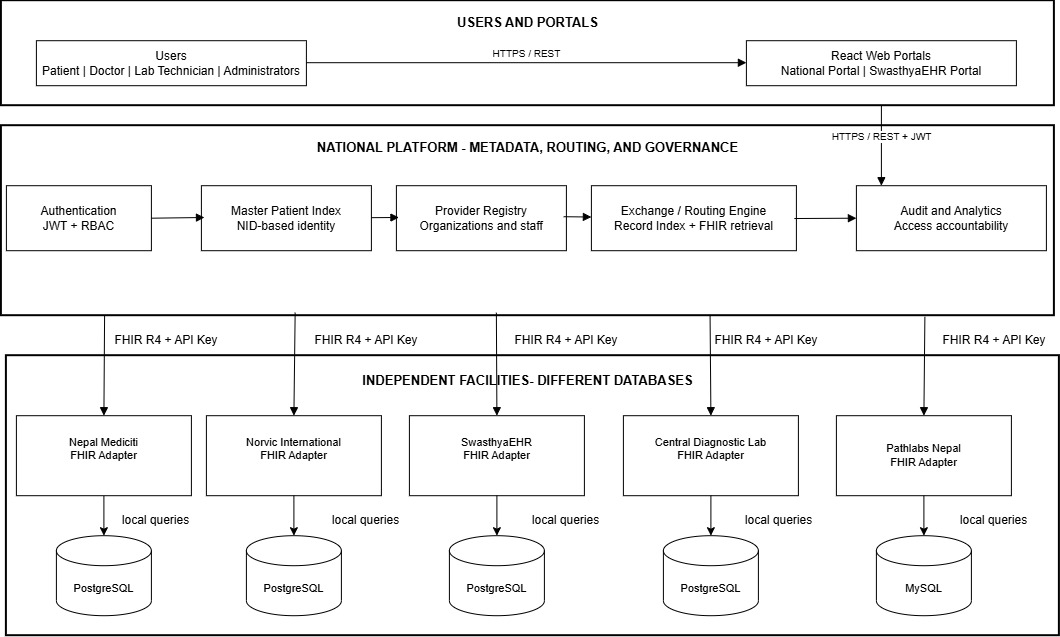
\includegraphics[width=1.3\textwidth,height=0.78\textheight,keepaspectratio]{Images/systemarcihtecture1.jpeg}%
}
\caption{Federated System Architecture}
\label{fig:architecture}
\end{figure}

The system architecture shown in Figure \ref{fig:architecture} follows a federated three-tier design. At the top, users access the system through a web browser; the National Frontend provides the user interface and communicates with the National Platform. In the middle, the National Platform, running on port 8000, stores only metadata and routing information: the Master Patient Index, the Provider Registry, the Record Index, and the Audit Log. It deliberately stores no clinical data. At the bottom, each participating facility maintains its own local database and exposes a read-only data interface through which the platform fetches clinical records on demand.

Security is enforced at two levels: users log in and are authorized based on their role, while organizations authenticate to the platform using unique API keys. Clinical data integrity is preserved by the federated design itself: the platform never stores clinical records, so a compromise of the platform cannot leak patient clinical data; it can only reveal that a patient has records at particular institutions.

\needspace{5\baselineskip}
\section{Use Case Diagram}
\begin{figure}[H]
\centering
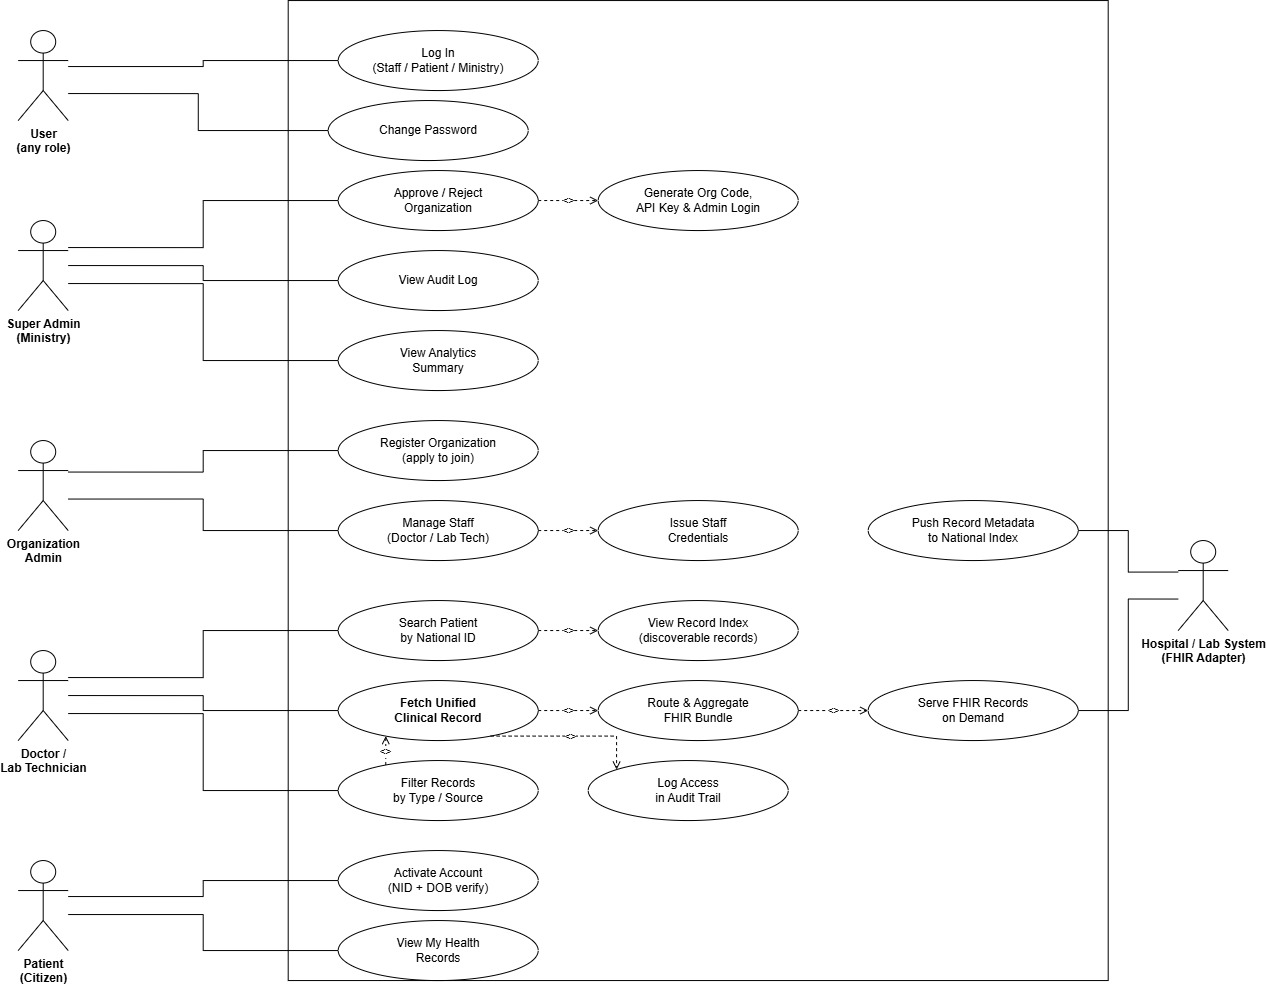
\includegraphics[width=0.95\textwidth]{Images/usecase1.jpeg}
\caption{Use Case Diagram of the System}
\label{fig:usecase}
\end{figure}

The use case diagram in Figure \ref{fig:usecase} models the interactions between six actors and the functions they perform within the Nepal Unified Health Record System. The actors are the System Administrator, the Super Admin (Ministry), the Organization Admin, the Doctor / Lab Technician, the Patient / Citizen, and the Hospital and Laboratory System. The diagram captures the full set of use cases supported by the system: logging in and changing passwords; activating accounts; registering organizations, approving or rejecting them; managing staff and issuing staff credentials; searching patients by National Identity Number; viewing patient records; querying aggregated health data and exporting data; and monitoring the system through the audit log and analytics dashboards.

Exchange-related capabilities are shared across actors: the Doctor / Lab Technician queries patient records and the hospital or laboratory system serves the requested records, so that every cross-institutional query depends on the data adapter exposed by each participating facility.

\section{Data Flow Diagram}
\subsection{Level 0 Data Flow Diagram}
\begin{figure}[H]
\centering
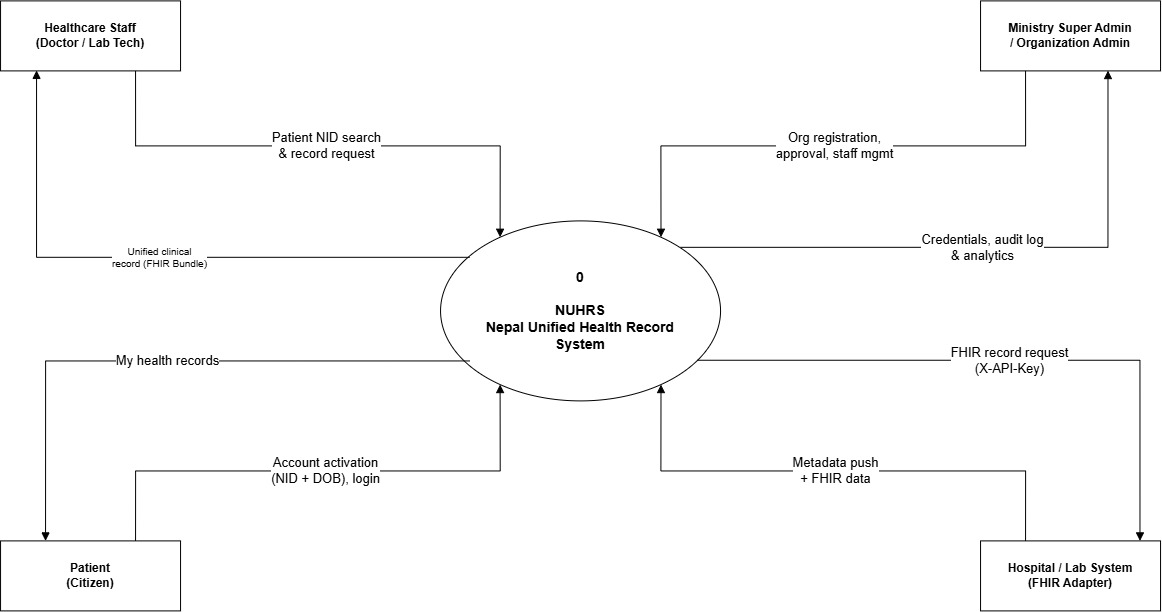
\includegraphics[width=\textwidth]{Images/dfd_level01.jpeg}
\caption{Level 0 Data Flow Diagram}
\label{fig:dfdlvl0}
\end{figure}

The Level 0 data flow diagram in Figure \ref{fig:dfdlvl0} provides the highest-level view of the Nepal Unified Health Record System, abstracting the entire platform as a single central process and showing its interactions with external entities. Two categories of external entities are depicted: (1) Healthcare Staff (Doctors and Lab Technicians), who initiate patient queries, submit record requests, and receive unified clinical records in return; and (2) the Ministry Super Admin and Organization Admin, who administer the platform by managing organization registrations, approving or rejecting participants, and monitoring national-level analytics and the audit trail. Internally, the platform maintains three persistent stores: the Master Patient Index, the Record Index, and the Audit Log while clinical data itself remains exclusively within the participating facilities and is fetched on demand through their data adapters. This diagram establishes the boundary of the system and the direction of data flows between actors and the central platform.

\clearpage
\subsection{Level 1 Data Flow Diagram}
\begin{figure}[H]
\centering
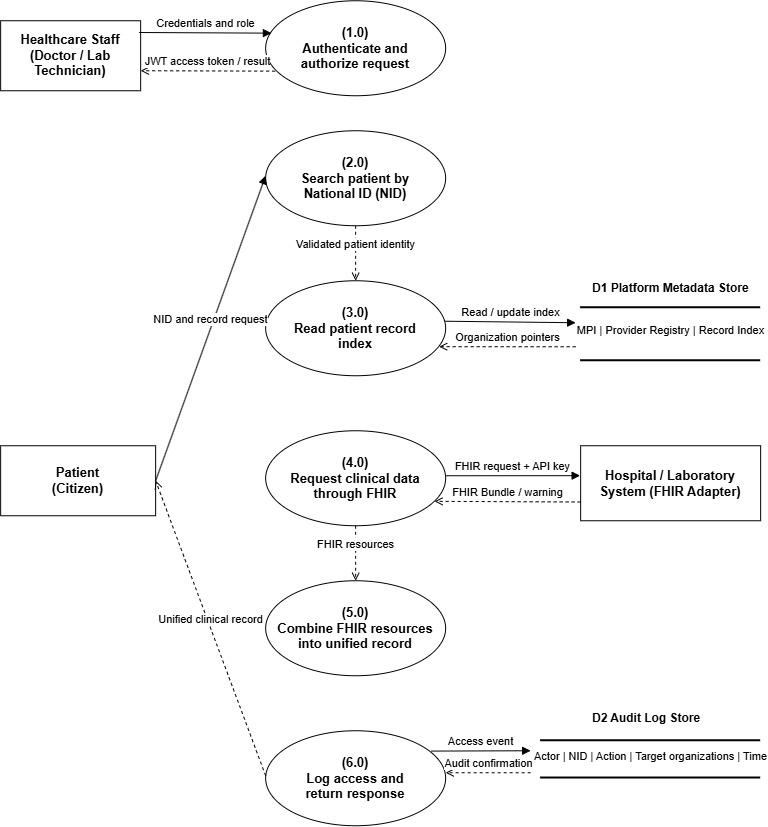
\includegraphics[width=\textwidth]{Images/DFD level 11.jpg.jpeg}
\caption{Level 1 Data Flow Diagram}
\label{fig:dfdlvl1}
\end{figure}

The Level 1 data flow diagram in Figure \ref{fig:dfdlvl1} decomposes the central process from the Level 0 diagram into its principal sub-processes, revealing the internal data flows that occur when a healthcare worker searches for a patient and retrieves a unified record. The key sub-processes depicted include: (1) Authentication and Authorization, where user credentials are verified and access tokens are issued; (2) Patient Identity Lookup, where the NID is validated and matched against the Master Patient Index; (3) Record Index Query, where the platform discovers which organizations hold records for the identified patient; (4) Data Retrieval, where the Routing Engine contacts each owning organization's data adapter to fetch clinical records; (5) Record Assembly and Normalization, where records from different organizations are merged into a single standardized collection; (6) Metadata Ingest, where organizations push record references to the national index; (7) Audit Logging, where every search, fetch, and administrative action is recorded; and (8) Organization Administration, where the Super Admin approves or rejects organization registrations. This diagram clarifies how data moves through the system at a detailed operational level.

\clearpage
\section{System Flowchart}
\begin{figure}[H]
\centering
\makebox[\textwidth][c]{%
    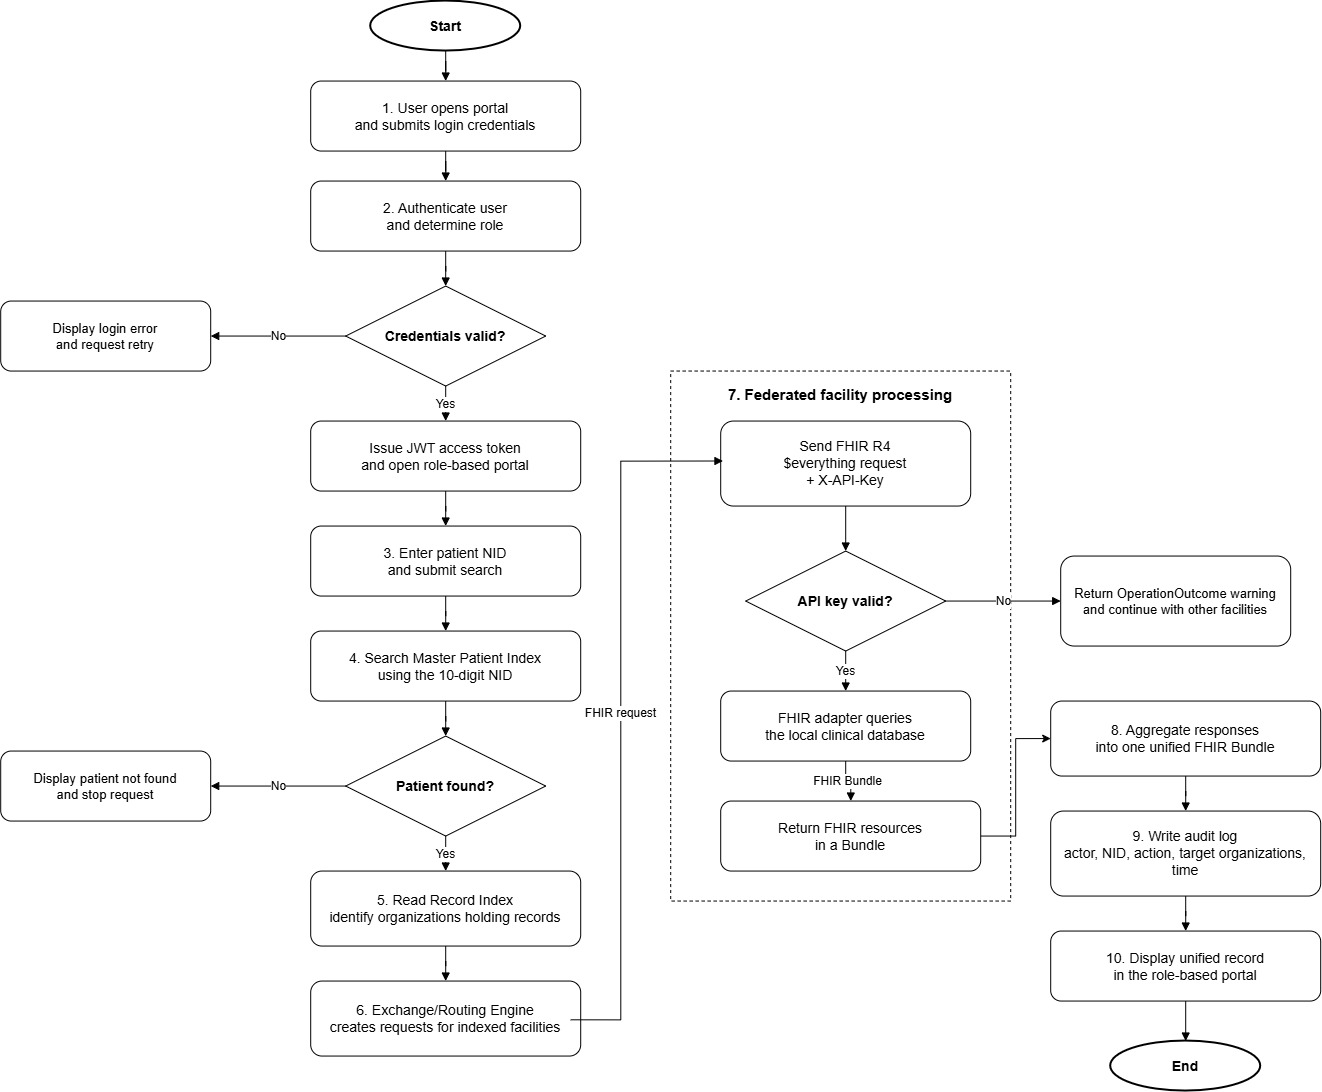
\includegraphics[width=1.1\textwidth,height=0.78\textheight,keepaspectratio]{Images/systemflowdiagram1.jpeg}%
}
\caption{System Flowchart}
\label{fig:flowchart}
\end{figure}

The system flowchart in Figure \ref{fig:flowchart} illustrates the complete operational path of the core exchange workflow from initiation to result delivery. The flow begins when a healthcare user (Doctor or Lab Technician) logs in and searches for a patient by National Identity Number (NID). The system validates the NID format; an invalid NID terminates the flow with an error message. For a valid NID, the platform queries the Master Patient Index and the Record Index to discover which organizations hold clinical records for that patient. If no records are found, an empty result is returned with an informational message. Otherwise, the Routing Engine contacts each owning organization's data adapter, retrieves all clinical records, and merges them into a single unified collection tagged by source facility. An audit log entry is written recording the actor, patient NID, contacted organizations, and timestamp. Finally, the system renders the unified record grouped by source institution and plots longitudinal trend charts for repeated clinical measurements such as blood glucose, HbA1c, blood pressure, and cholesterol.

\clearpage
\section{Entity-Relationship Diagram}
\begin{figure}[H]
\centering
\makebox[\textwidth][c]{%
    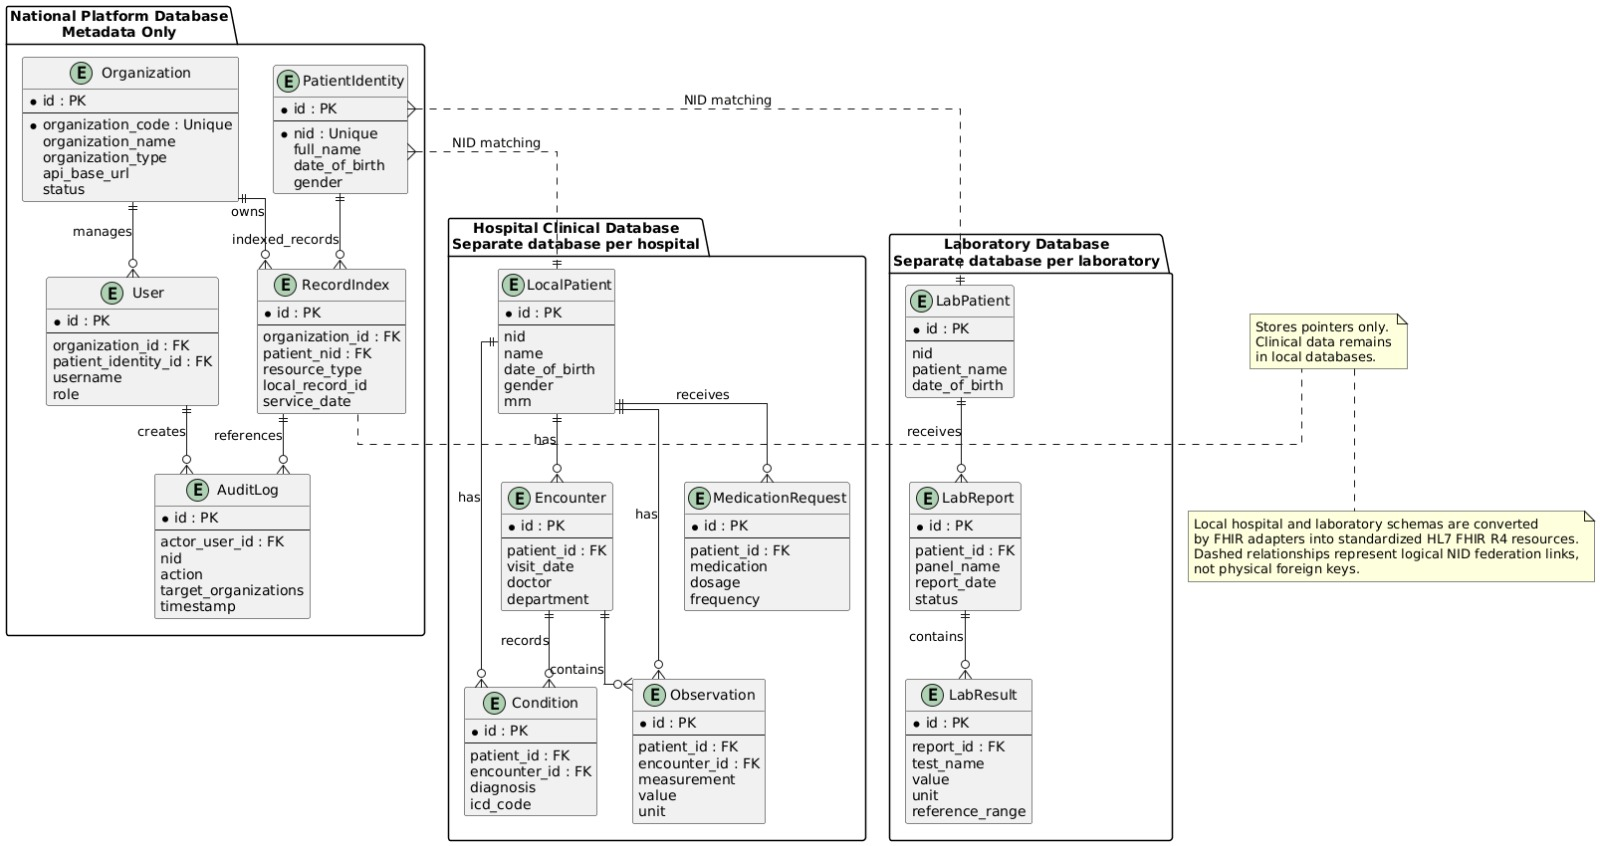
\includegraphics[width=1.1\textwidth,height=0.78\textheight,keepaspectratio]{Images/ER diagram1.jpeg}%
}
\caption{Entity-Relationship Diagram}
\label{fig:erdiagram}
\end{figure}

The Entity-Relationship (ER) diagram in Figure \ref{fig:erdiagram} models the data structure of the National Platform, showing the core entities, their attributes, and the relationships between them. The central entity is PatientIdentity (the Master Patient Index), which stores a patient's National Identity Number (NID) along with name, date of birth, gender, and contact information. Each PatientIdentity record is linked to one or more RecordIndex entries, which indicate that a particular organization holds specific records for that patient, together with a summary and the service date.

The Organization entity (the Provider Registry) stores each participating facility's name, type, license number, contact details, and registration status (pending, active, or rejected). The User entity supports the five system roles (Super Admin, Organization Admin, Doctor, Lab Technician, and Patient) with fields for username, role, and associated organization. The AuditLog entity records every cross-organization search and fetch operation, storing the actor, action type, patient NID, list of contacted organizations, timestamp, and IP address. The relationships depicted are: one PatientIdentity to many RecordIndex entries; one Organization to many RecordIndex entries; one Organization to many Users; and one AuditLog entry per access event. This data structure deliberately stores no clinical data on the National Platform only identity information, record references, and audit records, which is a fundamental design choice that preserves data sovereignty.

\section{Sequence Diagram}
\begin{figure}[H]
\centering
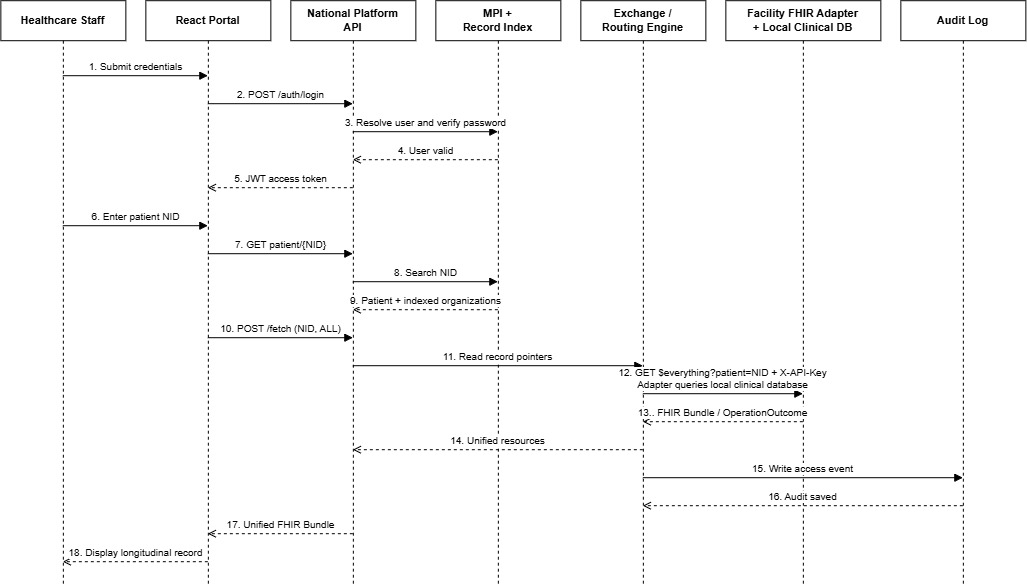
\includegraphics[width=\textwidth]{Images/sequencediagram1.jpeg}
\caption{Sequence Diagram of the Cross-Institutional Record Exchange Flow}
\label{fig:sequence}
\end{figure}

The sequence diagram in Figure \ref{fig:sequence} captures the step-by-step message exchange between the key participants during the cross-institutional record retrieval workflow. The participants depicted are the Doctor or Lab Technician (the requesting user), the National Frontend (the web interface), the National Platform (the central server), the Routing Engine (an internal component on the National Platform), and one or more Organization Services (hospital or laboratory data adapters).

The sequence begins when the Doctor logs in by sending credentials to the National Platform, which verifies them and returns an access token. The Doctor then initiates a patient search by NID through the frontend, which forwards the request to the National Platform. The platform checks the user's permissions, queries the Master Patient Index and Record Index to discover which organizations hold records for that NID, and returns the results to the frontend. When the Doctor triggers the fetch full unified record operation, the frontend sends the request to the National Platform, which delegates the operation to the Routing Engine. The Routing Engine identifies each owning organization, contacts their data adapters to retrieve clinical records, collects all responses, tags each record with its source organization, merges them into a single unified collection, writes an audit log entry, and returns the aggregated result to the frontend. The frontend then renders the unified record with source-grouped sections and longitudinal trend charts. If any organization is unreachable during this process, the Routing Engine returns a notification for that source rather than failing the entire request, ensuring graceful degradation.

\clearpage
\section{Security and Audit Flow}
\begin{figure}[H]
\centering
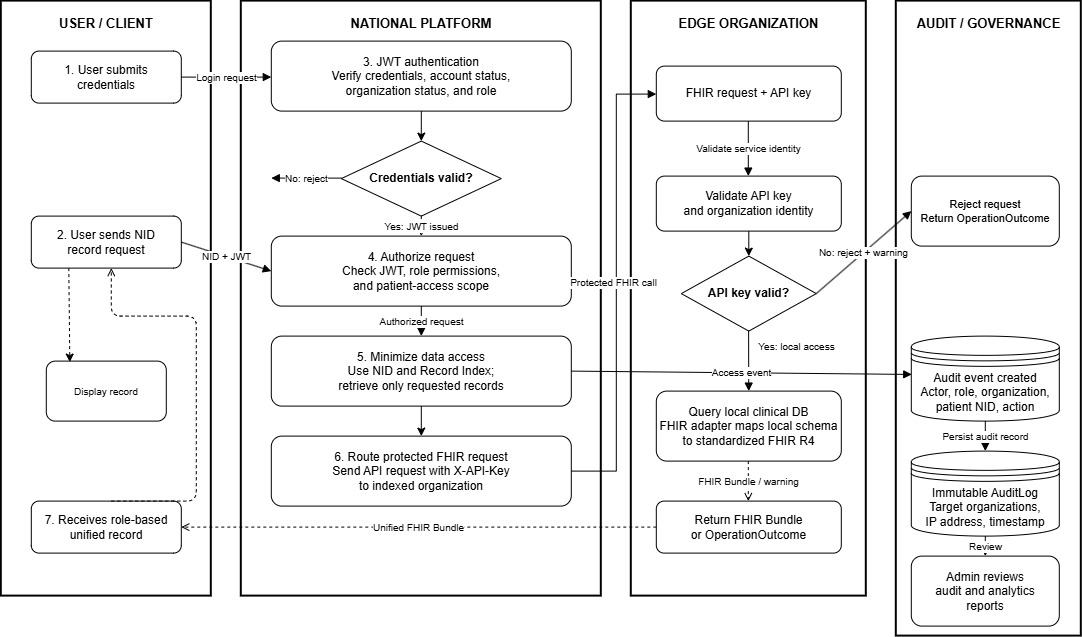
\includegraphics[width=\textwidth]{Images/securityandauditflow1.jpeg}
\caption{Security and Audit Flow}
\label{fig:securityaudit}
\end{figure}

The security and audit flow diagram in Figure \ref{fig:securityaudit} illustrates the security measures that protect data access at every point in the system. The diagram depicts two authentication pathways and the audit mechanisms that govern every cross-institutional data access event.

User Authentication: A healthcare user (Doctor, Lab Technician, or Patient) logs in through the National Frontend by submitting their credentials. The National Platform verifies the credentials, checks the user's role and organization scope, and issues a signed access token. All subsequent requests from the frontend carry this token. The platform validates the token and checks permissions on every request before returning any data. Patients are additionally restricted to their own records, so the system refuses to return records belonging to other patients.

Service-to-Service Authentication: When the Routing Engine contacts an organization's data adapter, it carries that organization's unique API key. Each organization validates this key before processing any request. If the key is missing, invalid, or belongs to a different organization, the request is rejected immediately.

Audit Trail: Every patient search and record fetch across the system is logged by the National Platform in an immutable Audit Log. Each log entry records who performed the action, what was done, which patient was involved, which organizations were contacted, the result status, the timestamp, and the user's IP address. The Super Admin can browse this full audit trail through the National Frontend dashboard, providing end-to-end accountability for all cross-institutional data access.

Data Sovereignty: The federated architecture itself serves as a security mechanism: because the National Platform stores only record references and never clinical data, a compromise of the platform cannot leak patient clinical records it can only reveal that a patient has records at particular institutions. Clinical data integrity is preserved by ensuring that each organization remains the sole authoritative source of truth for its own records, and no clinical data is ever copied into or cached by the central platform.

\clearpage
\section{Implementation Details}
\subsection{National Platform Backend}
The National Platform is built using the Django web framework and Django REST Framework, backed by PostgreSQL for data storage. Its data model is deliberately metadata-only, storing no clinical data. It maintains the Provider Registry (list of participating organizations), the Master Patient Index (minimal patient identity records), the Record Index (references indicating which organizations hold which records), a User model supporting the five roles, and the Audit Log. User authentication is handled through signed access tokens that expire after a fixed period, with newly created accounts requiring a password change on first login. Communication between organizations and the platform is authenticated using unique API keys.

\needspace{5\baselineskip}
\subsection{The Exchange and Routing Engine}
The Routing Engine is the central component responsible for retrieving unified patient records. Given a patient's National Identity Number, it consults the Record Index to determine which organizations hold records for that patient. It then contacts each organization's data adapter to retrieve the clinical records, merges all returned records into a single collection grouped by source organization, and writes an audit log entry. If any organization is unavailable, the system returns a notification for that source rather than failing the entire request, ensuring that partial results are still delivered.

\needspace{5\baselineskip}
\subsection{Hospital and Laboratory Data Adapters}
Each participating organization exposes a read-only data interface protected by an API key. To demonstrate the value of standardized data formats, the hospital and laboratory services deliberately use two different internal data structures, referred to as Variant A and Variant B. Despite these internal differences, each organization's adapter translates its local data into identical standardized FHIR resources: hospitals produce Patient, Encounter, Condition, Observation, MedicationRequest, and AllergyIntolerance resources; laboratories produce Patient and DiagnosticReport resources with laboratory observations coded using LOINC terminology; and Norvic International Hospital additionally provides Immunization and Procedure records. This approach proves that institutions with different internal systems can produce uniform, standardized output for exchange.

\needspace{5\baselineskip}
\subsection{Frontend}
The National Frontend is a web application served on port 3000. It provides role-specific views: a login and registration page; a Super Admin dashboard for organization approval, national analytics, and audit trail viewing; a Doctor and Lab Technician view for searching patients and retrieving unified records with longitudinal trend charts; and a read-only Patient Portal for viewing one's own records.

\chapter{Results and Discussion}

\needspace{5\baselineskip}
\section{Experiment setup}
The experimental setup consisted of the complete deployment described in the Hardware Configuration chapter: six application services, six databases, and two frontends running locally. The system was started, the National Platform automatically created the administrator account and approved the five demo organizations, and the seed script populated each hospital and laboratory with clinical records for the three shared demo patients.

The demonstration flow was then executed through the National Frontend: an Organization Admin created a Doctor login for Nepal Mediciti, the Doctor searched for patient Ram Bahadur Thapa by NID 12345678901, and the exchange view displayed the discoverable record index spanning both hospitals and both laboratories. Clicking fetch full unified record triggered the Routing Engine, which contacted all owning organizations and assembled a single unified record.

\section{Software Development Approach}
The Iterative Model proved suitable for the project because the system comprises independently developable components. The national platform, the hospital and laboratory services, the data adapter layers, and the frontend were developed in parallel across four iterations, with each iteration adding a new layer on top of working functionality. This approach allowed the team to identify and fix issues early, integrate components gradually, and refine the system throughout development.

\section{Deployment}
The complete system was packaged and deployed locally. The National Platform runs on port 8000, the hospitals on ports 8003 and 8004, the laboratories on ports 9001 and 9002, the SwasthyaEHR hospital on port 8090, and the frontends on ports 3000 and 3090. The deployment is fully scripted: the initialization command sets up the registry and credentials, and the seed script populates clinical data, so the entire environment can be started and recreated easily.

\needspace{5\baselineskip}
\section{Testing and Evaluation}
\subsection{Functional Validation}
The core exchange workflow was validated end to end. Searching NID 2345678901 returned the patient identity and a record index listing conditions, observations, medications, and allergies at Nepal Mediciti, Norvic International, and laboratory reports from both laboratories. The fetched unified record merged records from all sources into a single collection, with each record tagged by its source facility, even though the two hospitals store their data in different internal formats and one laboratory uses a different database system. This confirms that institutions with different internal systems can produce identical, standardized output for exchange.

\subsection{Longitudinal Trends}
The trends panel aggregated repeated measurements across institutions onto single timelines. For example, fasting blood glucose and HbA1c readings from Nepal Mediciti and serum creatinine readings from Norvic International were rendered as continuous trend charts with reference-range shading, and a toggle allowed filtering to measurements recorded at more than one facility. This demonstrates the clinical value of a federated record: a measurement recorded at several facilities appears on one timeline.

\subsection{Audit and Accountability}
Every search and record fetch was recorded in the audit log with the actor, action, patient NID, contacted organizations, and timestamp. The Super Admin dashboard displayed the full audit trail, and the analytics view reported totals for patients, records indexed, active organizations, and exchanges, along with top conditions and records by province.

\subsection{Security Validation}
Invalid NIDs were rejected at the system boundary, unauthenticated requests to protected endpoints were denied, organization API keys were verified on every service-to-service call, and patient-scoped endpoints refused to return records belonging to other patients. Organizations with invalid or missing API keys were denied access.

\subsection{Resilience Validation}
When a source organization was deliberately stopped, the Routing Engine returned a notification for that source while still returning all reachable records, confirming that a partial system degrades gracefully rather than failing entirely.

\chapter{Conclusions}
The Nepal Unified Health Record System project successfully designed and implemented a web-based prototype that enables organized, and on-demand sharing of patient health records across different healthcare institutions in Nepal. The system demonstrates that hospitals and laboratories can retain full ownership of their clinical data while a central National Platform, storing only patient identity information, record references, and access logs, enables authorized users to retrieve a unified patient record across all participating institutions.

The project achieved all of its stated objectives. A central web-based platform was developed that coordinates the discovery and retrieval of health records from participating organizations. Patients are uniquely identified across institutions using their National Identity Number, enabling records from multiple facilities to be linked under a single patient. A web portal with role-based access control allows different user types to perform their respective functions safely: administrators manage organizations and staff, doctors and lab technicians search for and retrieve patient records, and patients view their own records. A complete audit trail of all cross-institutional record searches and retrievals ensures accountability and traceability.

The experimental demonstration validated the core value of the approach: a clinician searching a single NID obtained a unified, longitudinal record spanning two hospitals and two laboratories, including cross-institutional trend charts that track health measurements over time. The project provides a practical blueprint for national health record interoperability in Nepal and demonstrates that existing standalone healthcare information systems can join the network through standardized data adapters, as proven by the integration of SwasthyaEHR as a third hospital.

\chapter{Limitations and Future Enhancement}
\needspace{5\baselineskip}
\section{Limitations}
\begin{itemize}
    \item The system has been demonstrated with a small number of simulated institutions and has not yet been tested with real healthcare organizations or formally validated against official data exchange standards.
    \item The system supports basic patient, visit, diagnosis, medication, allergy, and laboratory records but does not yet include imaging, referral letters, comprehensive practitioner information, or patient consent management.
    \item The prototype does not verify National Identity Numbers through the live government registration system or provide the encrypted communication and advanced credential management required for production deployment.
\end{itemize}

\needspace{5\baselineskip}
\section{Future Enhancement}
\begin{itemize}
    \item The system should be tested with real hospitals and laboratories and formally validated against official healthcare data exchange standards before wider deployment.
    \item The system should support imaging, referral letters, immunization, and other expanded record types with a consent mechanism that allows patients to manage access to their records.
    \item The system should integrate live National Identity Number verification, encrypted communication, and advanced credential management to meet production-level security requirements.
\end{itemize}

\addcontentsline{toc}{section}{References}
\renewcommand{\bibname}{References}
\bibliographystyle{unsrtquotes}
\bibliography{ref}

\chapter*{Appendices}
\addcontentsline{toc}{section}{Appendices}
\setcounter{figure}{0}
\renewcommand{\thefigure}{10.\arabic{figure}}
\noindent\textbf{Application Interface Screenshots}\\[0.5em]
\begin{figure}[H]
\centering
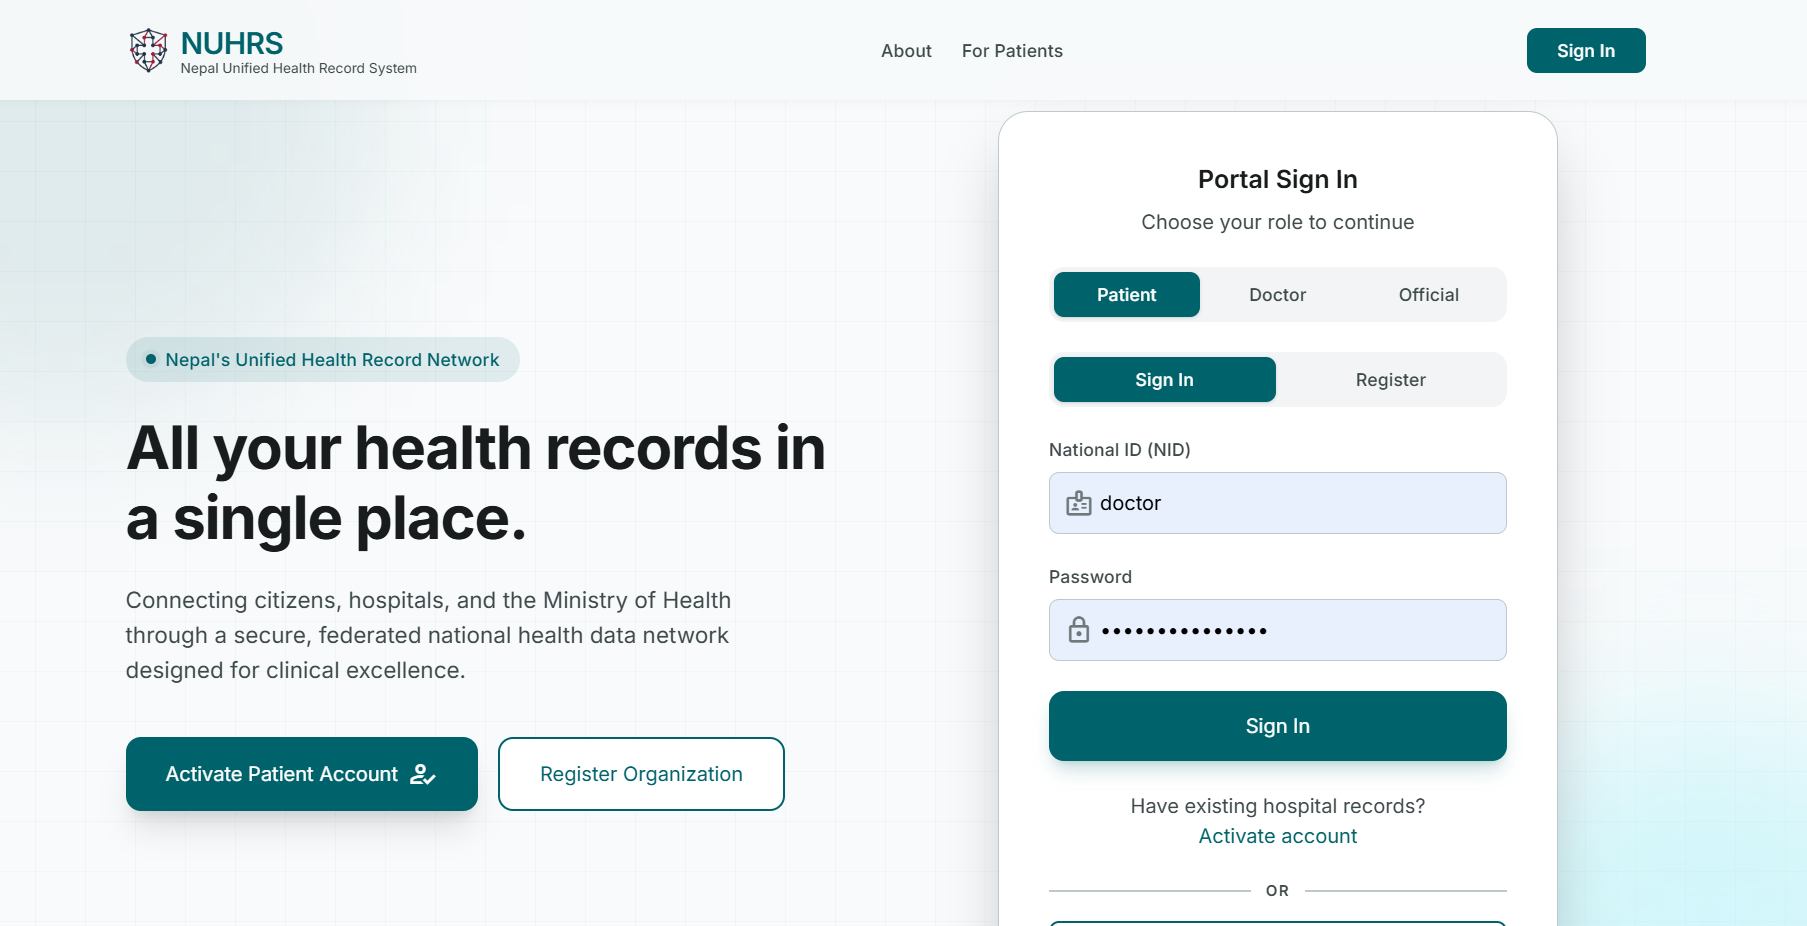
\includegraphics[width=0.8\textwidth]{Images/8.1 login page.png}
\caption{Login Page}
\end{figure}

\begin{figure}[H]
\centering
\begin{minipage}{0.48\textwidth}
\centering
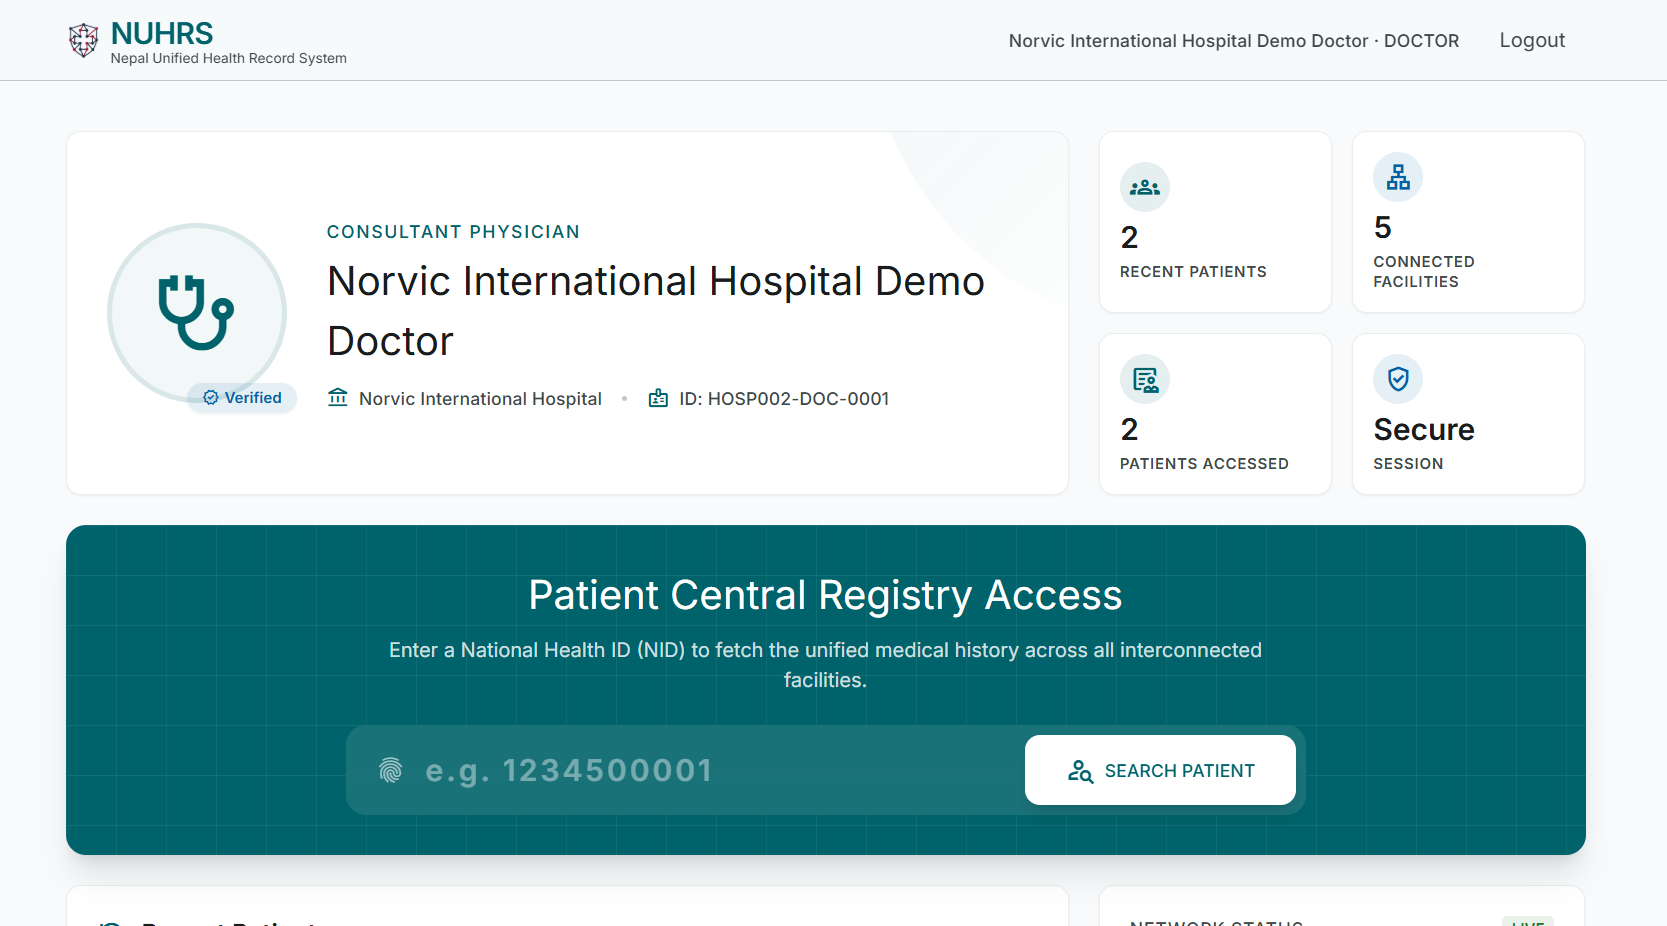
\includegraphics[width=\textwidth]{Images/doctor.png}
\end{minipage}\hfill
\begin{minipage}{0.48\textwidth}
\centering
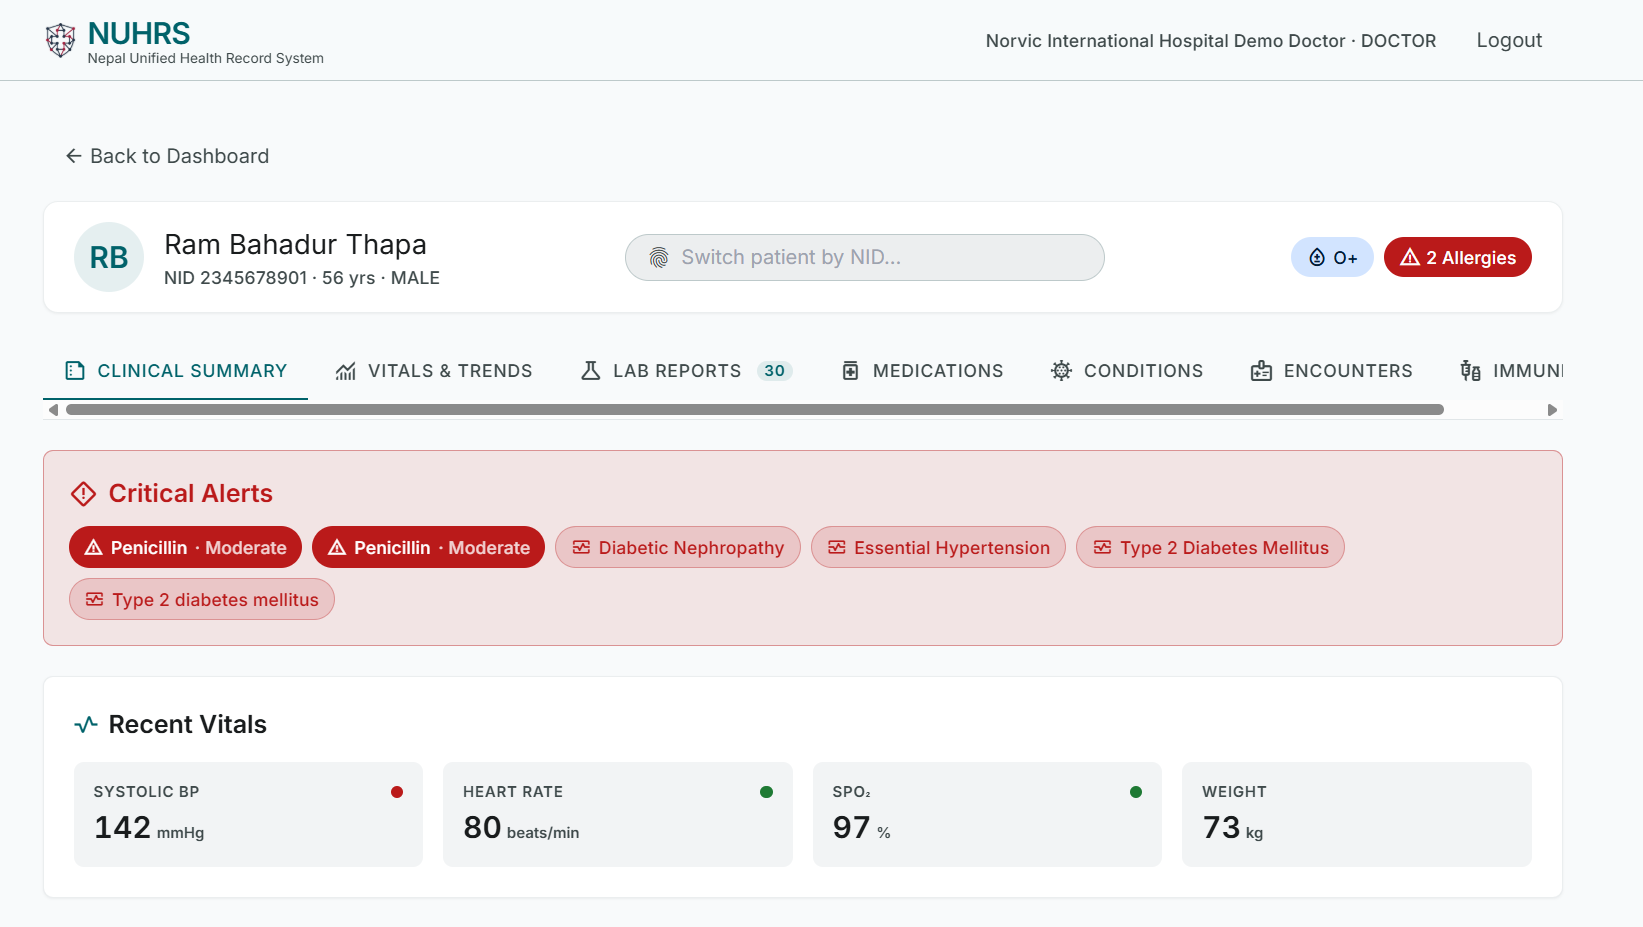
\includegraphics[width=\textwidth]{Images/8.2 doctordashboar2.png}
\end{minipage}
\caption{Doctor Dashboard}
\end{figure}

\begin{figure}[H]
\centering
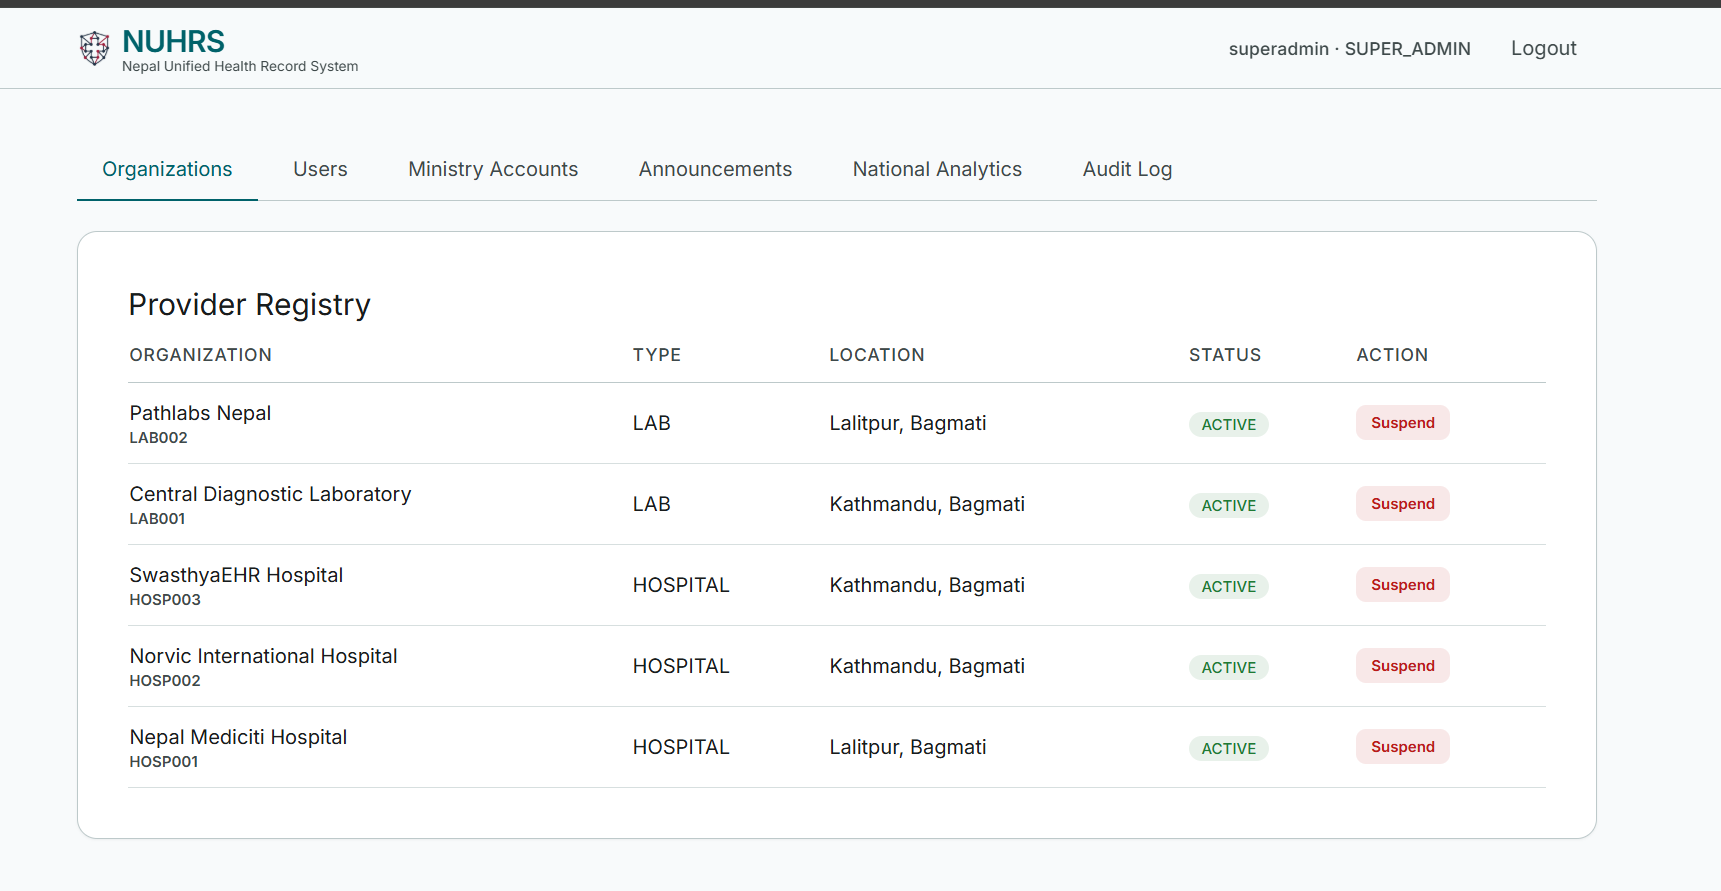
\includegraphics[width=0.8\textwidth]{Images/8.4 admin dashboard.png}
\caption{Admin Dashboard}
\end{figure}

\begin{figure}[H]
\centering
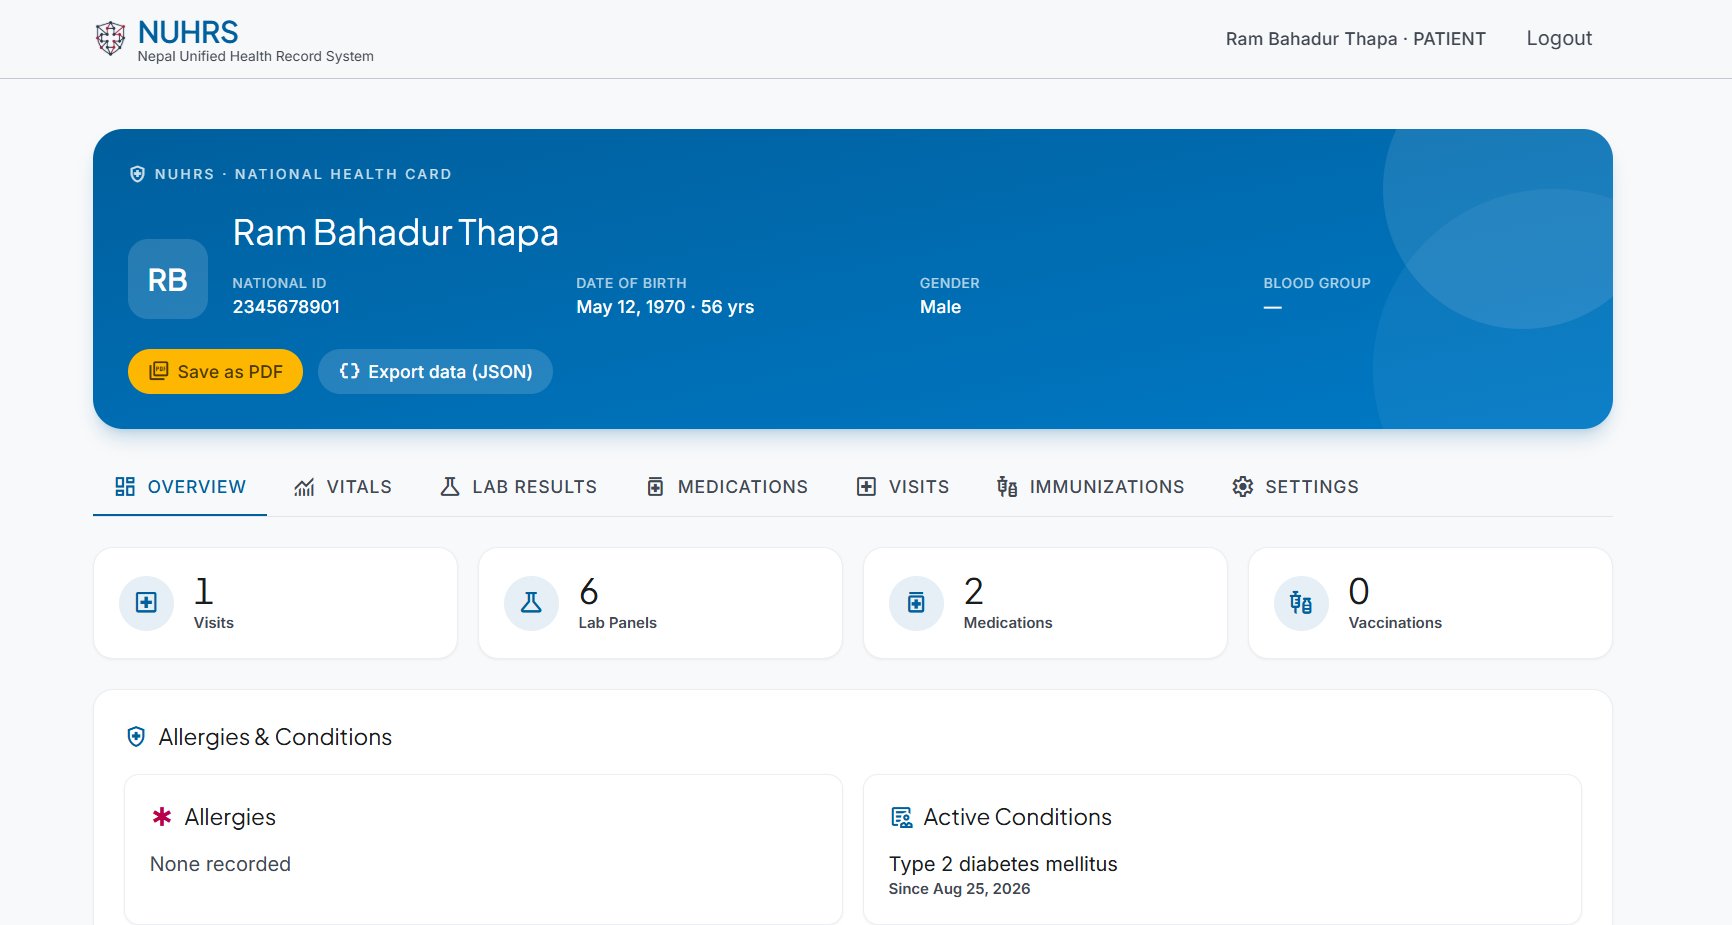
\includegraphics[width=0.8\textwidth]{Images/patient portal.png}
\caption{Patient Portal}
\end{figure}

\begin{figure}[H]
\centering
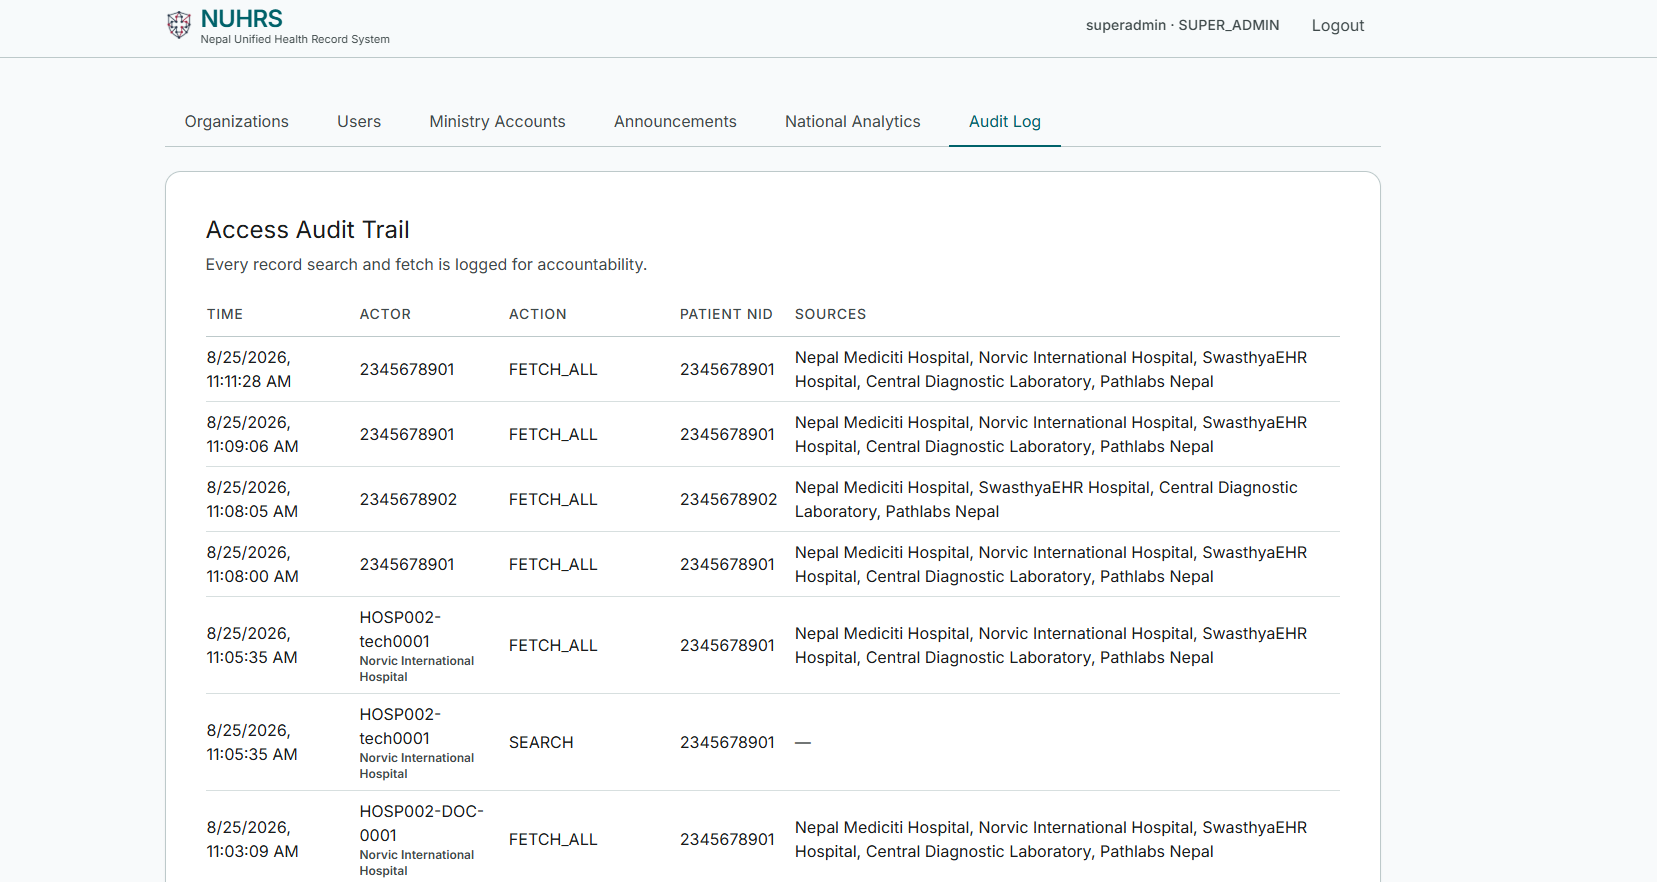
\includegraphics[width=0.8\textwidth]{Images/Figure 8.6 Audit Trail View.png}
\caption{Audit Trail View}
\end{figure}

\begin{figure}[H]
\centering
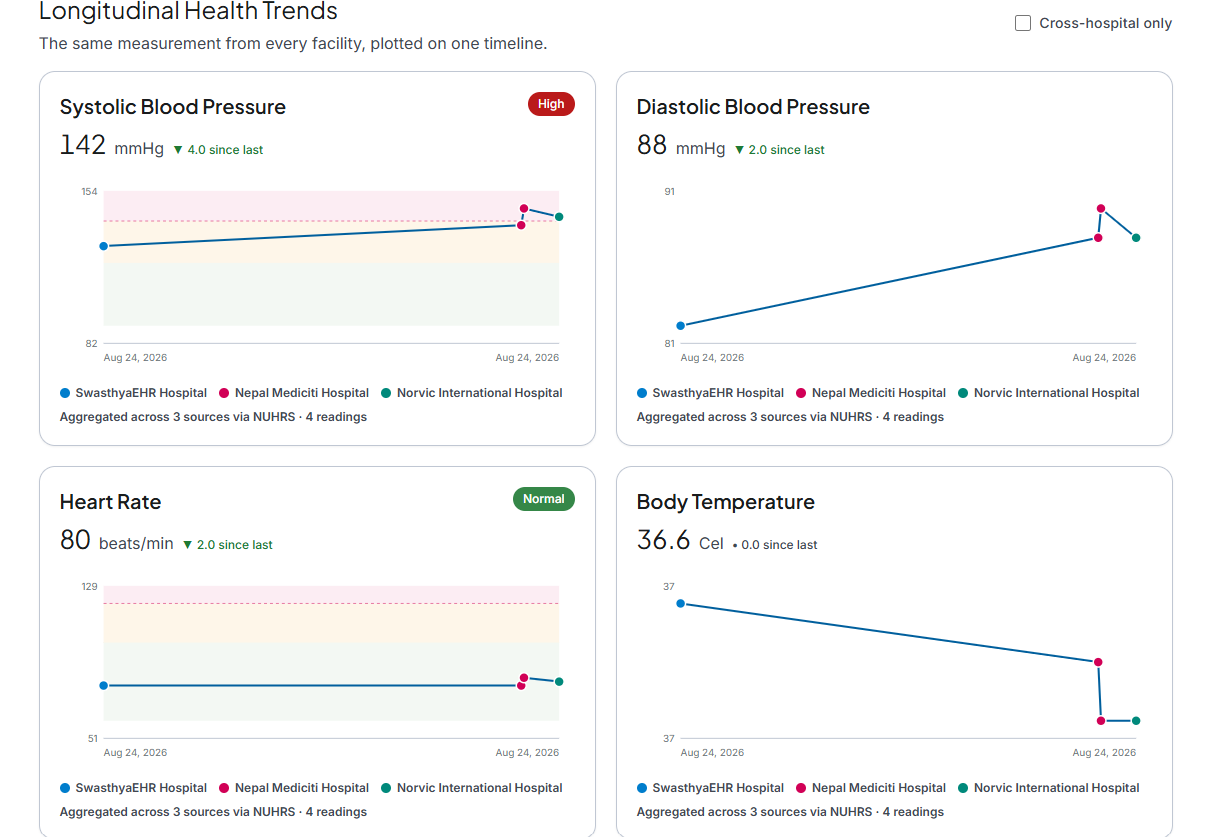
\includegraphics[width=0.8\textwidth]{Images/8.7 Longitudinal Trend Chart.png}
\caption{Longitudinal Trend Chart}
\end{figure}

\noindent\textbf{Demo Dataset}\\[0.5em]
The seeded federation uses three canonical demo patients shared across all institutions:\
\begin{tabular}{|p{3.2cm}|p{5.5cm}|p{3cm}|l|}
\hline
\textbf{NID} & \textbf{Name} & \textbf{DOB} & \textbf{Gender} \\ \hline
12345678901 & Ram Bahadur Thapa & 1970-05-12 & Male \\
12345678902 & Sita Kumari Sharma & 1988-11-23 & Female \\
12345678903 & Hari Prasad Koirala & 1979-02-03 & Male \\
\hline
\end{tabular}\\

Ram Bahadur Thapa carries Type 2 Diabetes Mellitus (E11.9) with serial fasting blood glucose and HbA1c readings at Nepal Mediciti, and Diabetic Nephropathy (E11.2) with serial serum creatinine readings at Norvic International. Sita Kumari Sharma carries Essential Hypertension (I10) with serial blood pressure readings. Hari Prasad Koirala carries Ischemic Heart Disease (I25.9) with serial LDL cholesterol readings. The demo data also includes Nepal-endemic conditions such as Dengue, Typhoid, Tuberculosis, Scrub typhus, and Hepatitis B, with matching laboratory panels. Norvic additionally contributes Immunization and Procedure records. The laboratory services contribute laboratory reports such as lipid profiles for the same patients.

\end{document}
